% +++++++++++++++++++++++++++++++++++++++++++++ CONFIGURATION ++++++++++++++++++++++++++++++++++++++++
% parameter for the print version (i.e. generate the blank pages added with \insertblankpage)
%  NB: the reason why it is featured is because the printed version, in some cases, should have the
%       part heading pages aligned on the RIGHT side ; then meaning that some blank pages are to be
%       inserted when a chapter does not have an even number of pages
%  NB: when using \insertblanpage, it will insert the page anyway ; it does NOT check the number of
%       pages of the part to compute if the page is required or not
\def\printversion{true}
% parameter to display appendices normally or simply the line in ToC
%  NB: this is useful if you do not want to include the appendices into the text but you want to keep
%       appendices lines in the ToC and also the labels for referencing
\def\displayappendices{true}
% Common parameters
\title{Penetration testing of commercial drones and realisation of a drone pentesting framework}
\author{Yannick PASQUAZZO}
\date{\today}
% Use and configure memoir class
\documentclass[11pt,a4paper,oneside]{memoir}
\setulmarginsandblock{2.5cm}{2cm}{*}
\setlrmarginsandblock{1.5cm}{1.5cm}{*}
%\renewcommand*\familydefault{\sfdefault} % use this to change overall font
\renewcommand*\familydefault{ppl}
% ++++++++++++++++++++++++++++++++++++++++++++++++++++++++++++++++++++++++++++++++++++++++++++++++++++
\checkandfixthelayout
% custom packages (contain all required usepackage's)
\usepackage{styles/thesis}
% ****************************** REMOVE BEFORE SUBMISSION - START ******************************
%\usepackage{draftwatermark}
%\SetWatermarkText{DRAFT}
%\SetWatermarkScale{1}
% ******************************* REMOVE BEFORE SUBMISSION - END *******************************
%
\makeindex
\makeglossaries
%
\begin{document}
  % include front cover page (MUST BE GENERATED FIRST!)
  
\includepdf[pages=1]{cover.pdf}
  \insertblankpage
  % content starts here
  \chapter*{Abstract}
\thispagestyle{empty}

\vspace{-3cm}
\vfill

\begin{center}
\begin{minipage}{15cm}
Nowadays, information security takes an increasing place in the world of Information Technologies. We work using software products provided by various companies all around the world, often assuming that these products are safe for use. Because of the rapid proliferation of Internet of Things in consumer and enterprise spheres over the last decade, the interest of malicious individuals consequently arises. Yet, security often comes second to functionality, without further thought of the possible consequences. 
\newline

To cope with this need in computer security, a new profession quickly arose : Penetration Tester. This job consists in testing the security of information systems ; because in order to know where you might have a breach, and patch it before it is exploited, the most efficient solution is to test the limits of your system yourself.
\newline

In particular, the drones are some of the most proliferating Internet of Things, being of interest for everyone, from children to seniors, from playing to working purposes. They range from cheap radio-guided toys, to very expansive GPS controlled tools, with of course the popular smartphone operated flying cameras. This allows a nefarious operator to snoop places that aren't supposed to be private, being the privacy of the neighbor's home or a government facility. But the drones aren't just hazardous because of the sensitive information they can reveal, they can also be used as weapons.
\newline

In this scope, our work aims to address the security of light commercial drones, to see if it is possible to break into the devices from a software point of view. To do so, we opted for an approach based on penetration testing in order to reveal the breaches, and then exploit those breaches to our advantage. We had no prior knowledge on the devices we tested, nor on the drone-related software development in general. We mostly relied on general IT background, as well as various tools developed by security professionals.
\newline

In this master thesis, we propose to apply some common hacking techniques and develop some exploit scripts to automate them. Ultimately, our contribution is to turn these scripts into modules for a brand new modular and extensible penetration testing framework in order to achieve penetration tests on drones in a structured and repeatable way. The framework is designed in the form of a command-line interface, mimicking the very popular toolkit called Metasploit. Being open source and modular, the framework hopes to catch the interest of drone security enthusiasts that are willing to contribute and develop exploits for more drone models in the future. 
\end{minipage}
\end{center}

\vfill

  \insertblankpage
  \chapter*{Foreword}
\thispagestyle{empty}

\vspace{-2cm}
\vfill

\begin{center}
\begin{minipage}{15cm}
\epigraph{``A nice quote."}{\textsc{John Doe \cite{manual-identifier}}}
\vspace{-1.2cm}
\hyphenation{wordthatshouldnotbehyphened}
Some text.

Some other text.

\end{minipage}
\end{center}

\vfill

  \insertblankpage
  \chapter*{Acknowledgements}
\thispagestyle{empty}

\vspace{-3cm}
\vfill

\begin{center}
\begin{minipage}{15cm}
I would like to express my gratitude to my supervisor, Captain Ir Alexandre D'Hondt, whose comments, advices and engagement through the period of my master thesis helped me to direct my efforts on rewarding matters. I would like to thank my tutor, Mr Ludovic Kuty, and Ir Pierre de Fooz for their guidance on troubleshooting some issues.
\newline

I would also like to thank my readers, Dr Ir Cyrille Mosbeux and Ing Thomas Guérin, who have kindly devoted their precious time for reading this thesis.
\newline

Furthermore, I would like to thank my entourage, for having supported me during this long and laborious process.
\end{minipage}
\end{center}

\vfill

  \insertblankpage
  % this part takes roman numerals page numbering
  \frontmatter
  \tableofcontents
  \insertblankpage
  \newacronym{is}{IS}{Information System}
\newacronym{ids}{IDS}{Intrusion Detection System}
\newacronym{ips}{IPS}{Intrusion Prevention System}
\newacronym{apt}{APT}{Advanced Persistent Threat}
\newacronym{va}{VA}{Vulnerability Assessment}
\newacronym{pt}{PT}{Penetration Test}
\newacronym{poc}{PoC}{Proof-of-Concept}
\newacronym{ptes}{PTES}{Penetration Testing Execution Standard}
\newacronym{cve}{CVE}{Common Vulnerabilities and Exposures}
\newacronym{cna}{CNA}{CVE Numbering Authorities}
\newacronym{iot}{IoT}{Internet of Things}
\newacronym{uart}{UART}{Universal Asynchronous Receiver Transmitter}
\newacronym{jtag}{JTAG}{Joint Test Action Group}
\newacronym{rtsp}{RTSP}{Real-Time Streaming Protocol}
\newacronym{ap}{AP}{Access Point}
\newacronym{crc}{CRC}{Cyclic Redundancy Check}
\newacronym{ssid}{SSID}{Service Set IDentifier}
\newacronym{bssid}{BSSID}{Basic Service Set IDentifier}
\newacronym{essid}{ESSID}{Extended Service Set IDentifier}
\newacronym{nic}{NIC}{Network Interface Card}
\newacronym{mitm}{MITM}{Man-In-The-Middle}
\newacronym{osint}{OSINT}{Open Source INTelligence}
\newacronym{jvm}{JVM}{Java Virtual Machine}

% then add all and print the list of acronyms
\glsaddall
\printglossary[style=customstyle,type=\acronymtype,title={List of Acronyms},toctitle={\textbf{List of Acronyms}}]
  \insertblankpage
  \listoffigures \addcontentsline{toc}{chapter}{\textbf{\listfigurename}}
  \insertblankpage
%  \lstlistoflistings \addcontentsline{toc}{chapter}{\textbf{List of Listings}}  %%%% ERROR
  % for the rest, page numbering is arabic
  \mainmatter
  \begin{chaptercover}{Introduction}%
{\coverepigraph{``When functionality is all that matters, security is often overlooked."}{\textsc{Alexandre D'Hondt} \newline {\normalsize\vspace{-.3cm}Cybersecurity expert at the Belgian Defense}}
{\large \hyphenation{} \bigletter{I}{nternet of Things} is on the rise with more than 30 billion devices connected worldwide expected by 2020. Today, controlling a device remotely has become the norm, especially through wireless protocols. Therefore, it is common to find light commercial drones which are controllable with a smartphone. As a result, malicious individuals might be tempted to leverage common security flaws. \newline \\ Proceeding from the general to the particular, this introduction reduces the scope to the field of security assessment, more exactly penetration testing. This chapter states the problem, highlights the desired objectives and approach and dissects the remainder of this document.\newline\\}}%
{introduction}

\begin{projectdata}
\begin{itemize}[labelsep=1cm]
  \item [\textbf{Domain}] Vulnerability Assessment \& Penetration Testing
  \item [\textbf{Scope}] Internet of Things : light commercial drones
  \item [\textbf{Audience}] Vulnerability Hunters
  \item [\textbf{Purpose}] Study the security of common light commercial drones and build a penetration testing framework based on the acquired knowledge
\end{itemize}
\end{projectdata}

\section{Problem Statement}
{\hyphenation{generally}
The past few years, more and more connected devices have invaded our daily lives. Although this generally allows us to improve our living environment, the proliferation of these connected gadgets is not without consequences. Indeed, each of these devices can be remotely controlled, either from the Internet or in their vicinity, which implies obvious security risks. More specifically, this work focuses on some ways an attacker could break into light commercial drones and the impact it could have. To name a few, a malicious person might be able to eavesdrop the video of a device, steal or even crash it.}

Some companies have already developed some commercial products in order to provide protection against drones threatening safety, security and privacy. Some of these solutions are as simple as firing a net to catch a device or disrupting the signal by emitting interference and thus making a drone inoperable. Some more advanced technologies also tackle the problem by sending specific commands to force a landing or make a drone go back to a certain point.

But, as far as we know, in the scope of drone software security, there still lacks a convenient open-source solution for gathering and coordinating exploits, one toolkit such as Metasploit, which is already well-established regarding OS penetration testing. That is what we propose in this master thesis; we try, first, to develop several exploits working on the drones we were provided, then we create an open source framework that we design to be modular and easy to contribute to.


\section{Objectives}
Our objectives are four-fold :
\begin{enumerate}[itemsep=0.2cm,topsep=0.1cm]
  \item State the \textbf{background}.
  \begin{enumerate}[label=\Alph* --,align=left,itemsep=.1cm]
    \item Review the current literature about IT security and especially IoT security.
    \item Search for processes and methodologies for hacking systems.
    \item Browse some existing solutions and tools and select relevant ones for exploitation.
  \end{enumerate}
  \item Narrow our \textbf{scope}.
  \begin{enumerate}[label=\Alph* --,align=left,itemsep=.1cm]
    \item Select some models of light commercial drones based on their technology.
    \item Filter out WiFi-based drones and understand their working.
  \end{enumerate}
  \item Build some \textbf{exploits} for breaking into the selected drones.
  \begin{enumerate}[label=\Alph* --,align=left,itemsep=.1cm]
    \item Find attack chains for the selected models of drones.
    \item Design and implement short scripts for exploiting found security holes.
  \end{enumerate}
  \item Put it altogether in a \textbf{framework}.
  \begin{enumerate}[label=\Alph* --,align=left,itemsep=.1cm]
    \item Set the basis for the framework.
    \item Turn the exploits into reusable modules.
  \end{enumerate}
\end{enumerate}

\section{Approach}
The school provides some criteria related to the scientific and technological content that are worth being parsed regarding our approach. Succinctly, these criteria match our approach like follows :
{\hyphenation{}
\begin{enumerate}[itemsep=0.1cm,topsep=0.1cm]
  \item {\color{FirstBlue}\bfseries Problem analysis} : From general to particular, we narrow our scope to a few targets and clearly state the requirements for the deliverables.
  \item {\color{FirstBlue}\bfseries Solution provided} : We implement the requirements into exploit scripts and ultimately a penetration testing framework tailored to drone hacking.
  \item {\color{FirstBlue}\bfseries Rigor of the approach} : We segment our approach from the state-of-the-art knowledge to measurable and assessable practical outcomes.
  \item {\color{FirstBlue}\bfseries Innovation} : We provide a brand new solution, gather and leverage the best of the parsed and acquired knowledge.
  \item {\color{FirstBlue}\bfseries Personal contribution} : We develop exploit scripts and modules for the new penetration testing framework.
  \item {\color{FirstBlue}\bfseries Avenues for future development} : We provide an extensible solution that could stir up the curiosity of drone hacking enthusiasts.
\end{enumerate}}

Regarding the skills acquired during our formation at the school, this project mainly applies, directly or indirectly, the following courses :
\begin{itemize}[itemsep=0.1cm,topsep=0.1cm]
  \hyphenation{}
  \item{} [{\color{FirstBlue}\bfseries B38}] Operating systems and introduction to IoT : By learning the basics of the Linux operating system and therefore allowing to have a better understanding of the architecture of the drones.
  \item{} [{\color{FirstBlue}\bfseries M18}] Network programming and software security : By using the acquired knowledge and tools related to network protocols to develop exploits that can be used from a distance. Cryptography knowledge were also a must-have.
  \item{} [{\color{FirstBlue}\bfseries M18}]  Internet of Things : Because it is the main subject of this thesis, and, in addition to this, the course strongly insisted on penetration testing and security.
  \item{} [{\color{FirstBlue}\bfseries M18}] Network security : By having prior knowledge of the specifics of network security, such as safe connection to a remote host.
  \item{} [{\color{FirstBlue}\bfseries M28}] Study of wireless networks : By applying the knowledge of the 802.11 protocol, we order to successfully capture and decrypt WiFi transmissions.
  \item{} [{\color{FirstBlue}\bfseries M18+M28}] Communication and language : By writing the thesis in English, thus increasing the scope of readers.
\end{itemize}

\section{Content}
The remainder of this document is structured as follows :
\begin{itemize}[itemsep=0.1cm,topsep=0.1cm]
  \item \hyperref[background]{\color{FirstBlue}\bfseries Chapter 2 -- Background} provides background information in the field of IT security and especially drone hacking. It explains a popular methodology, some techniques and outlines a few existing solutions, either commercial or open-source.
  \item \hyperref[scope]{\color{FirstBlue}\bfseries Chapter 3 -- Scope} presents some models of drones and their overall working, fixing the scope of this thesis to a few targets.
  \item \hyperref[exploits]{\color{FirstBlue}\bfseries Chapter 4 -- Exploits} explains the applied hacking techniques and their related exploit scripts.
  \item \hyperref[framework]{\color{FirstBlue}\bfseries Chapter 5 -- Framework} presents the drone penetration testing framework and its modules, developed from the aforementioned exploit scripts.
  \item \hyperref[conclusion]{\color{FirstBlue}\bfseries Conclusion} closes this introduction by presenting a general summary, by parsing the achieved objectives and outcomes of this work and by providing ways ahead and ideas for future works.
\end{itemize}


\section{Conventions \& Reading Advices}
This document is organized in such a way that it can be read mostly using a method in three passes. Indeed, the reader who wants to spare time can get an insight of this work, as a first pass, by solely reading the chapter cover pages. The reader who can take a bit more time for this reading, as a second pass, can directly jump to the end of the chapters for reading the summaries and discussions. Ultimately, the interested reader, as a third pass, can read the entire content.

\begin{tip}
\hyphenation{quotation contain chapters}
\vspace{-.5cm}
\paragraph{Why such a layout ?}\hfill

In order to get this document as much attractive as possible, we designed it with an unusual style, starting each chapter with a cover page providing a quotation from an IT professional and introducing the chapter matter bouncing from the quotation. We hope the reader will enjoy reading it !

\paragraph{Want to spare time ?} \hfill

Check the summaries and related discussions at the end of each chapter, they contain information enough so that one can quickly get the main thread !

\paragraph{More focused on Drone Hacking ?} \hfill

Check chapters \hyperref[background]{\color{FirstBlue}\bfseries 2} and \hyperref[scope]{\color{FirstBlue}\bfseries 3} then look at the summaries and related discussions of chapters \hyperref[exploits]{\color{FirstBlue}\bfseries 4} and \hyperref[framework]{\color{FirstBlue}\bfseries 5}.

\paragraph{More focused on the Exploitation Framework ?} \hfill

Check chapters \hyperref[exploits]{\color{FirstBlue}\bfseries 4} and \hyperref[framework]{\color{FirstBlue}\bfseries 5} and their related appendices.
\end{tip}

\end{chaptercover}

%  \insertblankpage
  \begin{chaptercover}{Background}%
{\coverepigraph{``I believe that the challenges of IT security will continue to increase, even if the operating systems and applications drastically improve."}{\textsc{H. D. Moore} \newline {\normalsize\vspace{-.3cm}Cybersecurity expert, developer of Metasploit}}
{\large \hyphenation{} \bigletter{I}{T security} is nowadays a very flourishing field with the evolution of technologies, bringing new challenges and techniques, especially when trying to break into systems. \newline \\ This chapter presents some basics about penetration testing, the ultimate science of breaking into systems, starting with defining what a penetration test is, then explaining the different test levels, methodologies and techniques as of the current state-of-the-art. It then lists a few existing tools in this field.\newline\\}}%
{background}

\section{Terminology}

Several notions should be known before continuing. This section defines the most important ones with their distinctions when relevant.

\subsection{Vulnerability VS Weakness}\label{subsec:vuln-vs-weakness}

In order to emphasize the difference between weaknesses and vulnerabilities, we use the definitions of MITRE. \cite{mitre}

\paragraph{Weaknesses} \textit{are flaws, faults, bugs and other errors in software implementation, code, design, or architecture that if left unaddressed could result in systems and networks being vulnerable to attack. Example of software weaknesses include but are not limited to: buffer overflows}, user interface errors, path name traversal, authentication errors, hardcoded credentials. \cite{mitre-cwe}

\paragraph{Vulnerabilities} are a consequence of weaknesses that are already present in the code. \textit{A software vulnerability, such as those enumerated on the \acrfull{cve} ® List, is a mistake in software that can be directly used by a hacker to gain access to a system or network.} \cite{mitre-cwe}

\paragraph{\acrfull{cve} ®} is a list of common identifiers for publicly known vulnerabilities.

\textit{Use of CVE entries, which are assigned by \acrfull{cna} from around the world, ensures confidence among parties when used to discuss or share information about a unique software or firmware vulnerability, provides a baseline for tool evaluation, and enables automated data exchange.} \cite{mitre-cve}

\textit{By definition, \acrshort{cve} is :
\begin{itemize}[itemsep=0.1cm,topsep=0.1cm]
  \item One identifier for one vulnerability or exposure
  \item One standardized description for each vulnerability or exposure
  \item A dictionary rather than a database
  \item How disparate databases and tools can "speak" the same language
  \item The way to interoperability and better security coverage
  \item A basis for evaluation among services, tools, and databases
  \item Free for public download and use
\end{itemize}}

\subsection{Black VS White hat hacker}

\paragraph{Blackhat hacker (the {\color{venetianred} Bad})} This profile is the malicious guy who wants to break into systems for his own benefit, in general for financial reasons.

\paragraph{Whitehat hacker (the {\color{forestgreen(web)} Good})} This profile pertains to the security expert and/or researcher who searches for security issues in \acrshort{is}' and whose goal is to fill the security gaps.

\begin{info}
In the scope of this work, we act as whitehat hackers as our project aims to identify and help fix security issues on light commercial drones.
\end{info}

\subsection{Kinds of assessment}

\paragraph{Penetration Testing} \textit{... can be defined as a legal and authorized attempt to locate and successfully exploit computer systems for the purpose of making those systems more secure.} \cite{basics-of-hacking-and-pt} The main idea is to find security issues just like an attacker would do so that these can be mitigated before a real attack.

\paragraph{\acrfull{va}} This kind of security assessment is a system review aimed to find potential security issues, generally performed in a live environment. The important point here is that it stops after having found vulnerabilities and reported them for mitigations, it does not assess their exploitability yet. At some point, when reported vulnerabilities are too numerous, it could be helpful to focus attention on these that could be effectively exploited for breaking into the related \acrshort{is} and direct the available resources on fixing these issues instead of trying to fix all the reported vulnerabilities (whose most of them are often informational or very difficult to exploit in practice). This is what distinguishes a \acrlong{va} from a \acrlong{pt}.

\paragraph{\acrfull{pt}} This kind of security assessment encompasses the \acrshort{va} but goes far beyond, demanding more resources (in time and efforts) to check for the exploitability of the found vulnerabilities in order to determine with more precision their impact on \acrshort{is}' environment. The outcome of such a test is a \textbf{\acrfull{poc} attack} that demonstrate the exploitability. This can lead to the discovery of security holes opening the way to pervasive actions like listed hereafter. The most important point here, and what distinguishes a penetration tester from a real attacker, is the \textbf{permission} (nonwithstanding the difference in motivation).

Multiple effects can result from the exploitability of a vulnerability :
\begin{itemize}[itemsep=0.1cm,topsep=0.1cm]
  \item Sensitive or even critical business-related data exfiltration.
  \item Potential for service and system disruption, that could lead to heavy financial impact for the host organization.
  \item Pivoting inside organization's network to impact other systems than the original target \acrshort{is}.
\end{itemize}

Ultimately, the main purpose of these kinds of security assessments is to report on security holes to the management, to provide mitigations and recommendations and to prioritize them in order to prevent real attacks from being led.

\paragraph{Red teaming} This notion pertains to simulating what we could begin to describe as an \acrfull{apt}. In this context, the \acrshort{pt} is extended over a much larger period (several months instead of a few days or weeks). This kind of scenario is more rare, as it demands far more resources to be carried out. However, this reflects even more closely the context of an external attack in which hackers increasingly tend to take their time to study the targeted \acrshort{is} and also to hide their presence.

\paragraph{Vulnerability hunting} This notion also refers to system or software review, but generally on a product outside its operating environment. It pertains to studying an asset in order to demonstrate its potential security flaws and help the manufacturer fix them before or yet after its deployment on the market.

\begin{info} \hyphenation{manufacturers}
In our case, we use the penetration testing approach and its related techniques to achieve vulnerability hunting on multiple drone models from various manufacturers.
\end{info}

\section{Types of penetration test}

A penetration test can take a different form according to the requirements of the target organization, the assessment depth and the degree of starting information. Figure \ref{fig:pentest-types} depicts the different types in function of the degree of prior knowledge.

\begin{figure}[H]
  \centering
  
\includegraphics[width=.7\linewidth]{figures/pentest-types}
  \caption{Types of penetration test in function of the prior degree of knowledge}
  \label{fig:pentest-types}
\end{figure}

\subsection{Blackbox}

A black box is the representation of a system taking inputs and giving outputs, with no consideration of its internal functioning. This working is either inaccessible (simply not available or lost), or deliberately omitted (in order to simulate the conditions in which a real attacker would operate).

In the \textit{Blackbox} context, the pentester really puts himself in the shoes of an external attacker and starts his penetration test with as little information as possible on his target (his target then being the company having requested the assessment). Indeed, when the tester begins his attack, he does not have (or rarely) the complete map of the \acrshort{is}, the list of servers with their IP, and so forth. The \textit{Blackbox} context aims to find and demonstrate the presence of an actionable plan by an external person to take control of the \acrshort{is} or get hold of certain information.

Reasons for black box penetration testing :

\begin{itemize} \vspace{-.2cm}
  \item[\checkmark] Simulates the majority of potential attacks facing your organization
  \item[\checkmark] Helps to identify where your systems are weakest
  \item[\checkmark] Provides an objective, outsider’s view of your systems
\end{itemize}

\subsection{Whitebox}

In systems theory, a white box, is a module of a system that can be expected to work internally because we know the operating characteristics of all elements that compose it. In other words, a white box is a module that has as few black boxes as possible.

In this case, the pentester works in close collaboration with the DSI, the RSSI and the technical team of the information system. The goal is to obtain 100\% information on the information system and to support the CIO in the detection of vulnerability. One of the advantages of the White Box mode is that it is then possible to detect security flaws in a wider way and that the Black Box mode would not have made it possible to detect, for example if the pentester had not reached a certain stage of the intrusion. In addition, the White Box mode is more easily integrated into the \acrshort{is} lifecycle, sometimes at each stage of its evolution.

Reasons for white box penetration testing:
\begin{itemize} \vspace{-.2cm}
  \item[\checkmark] Efficient use of ethical hacker’s time
  \item[\checkmark] Provides “full disclosure” insights
  \item[\checkmark] Allows for objective scrutiny of internal systems
\end{itemize}

\subsection{Greybox}

An engagement that allows a higher level of access and increased internal knowledge falls into the category of gray-box testing. Comparatively, a black-box tester begins the engagement from a strict external viewpoint attempting to get in, while the gray-box tester has already been granted some internal access and knowledge that may come in the form of lower-level credentials, application logic flow charts, or network infrastructure maps. Gray-box testing can simulate an attacker that has already penetrated the perimeter and has some form of internal access to the network.

By providing some form of background to the security consultants undertaking the assessment, it helps to create a more efficient and streamlined approach. This saves on the time (and money) spent on the reconnaissance phase, allowing the consultants to focus their efforts on exploiting potential vulnerabilities in higher-risk systems rather than attempting to discover where these systems may be found.

Reasons for grey box penetration testing :
\begin{itemize} \vspace{-.2cm}
  \item[\checkmark] Focus the attention on more highly-valuable areas within the network
  \item[\checkmark] Increases the attack coverage and efficiency
  \item[\checkmark] Cost effective
\end{itemize}

\begin{info} \hyphenation{}
The point here is that the type of testing we will achieve will depend on the target, as only a few information or even none could be available. We will see that some models of target and their related manufacturers are not always very transparent, then forcing the test to be limited to blackbox.
\end{info}

\section{Methodology, disciplines \& techniques}

This section presents the chosen methodology and some disciplines and techniques that will be used in the remainder of this work.

\subsection{\acrlong{ptes}}

After having introduced what is a pentest, let us look at a popular methodology for organizing a pentest.

\begin{question}
\textbf{But why do penetration testers need to follow a methodology ?}
\begin{itemize}
  \item The world is changing fast, security techniques and technologies are constantly evolving. Faced with this, \textbf{structure} is needed. The methodologies allow to provide a fixed framework on the progress of a penetration test.
  \item Faced with an \acrshort{is} or many, a pentester has to look into each system, service, port or IP which can hide a vulnerability ; this cumbersome and error-prone. A framed and fixed methodology then makes it possible to follow a \textbf{canvas} and thus to organize the penetration test so that it is as \textbf{complete} as possible and \textbf{repeatable}.
  \item In the professional environment, \textbf{team working} is essential. A methodology known by several pentesters will facilitate the work within the team. Also, the report generated will be made following a known frame.
\end{itemize}
\end{question}

First and foremost, a methodology will make it possible to not forget anything during the penetration test and to make sure that it is as complete as possible. During said pentest, the methodology acts as a way to follow, facilitating the organization of the pentester.

\paragraph{\acrfull{ptes} \cite{ptes}} Let's take a look at this popular methodogy that is often used by most pentesters. Mostly, this methodology is used as a basis in the pentest teams who customize them with their own methods, tools and techniques, which is what will make the difference between one team of pentest and another. The experience of the field is then added to the theory of the methodology. It should also be noted that each pentest follows a path of its own according to the \acrshort{is} to be tested. This methodology follows the steps as depicted in \ref{fig:ptes-process} and explained hereafter.

\begin{figure}[H]
  \centering
  
\includegraphics[width=\linewidth]{ptes-process}
  \caption{\acrshort{ptes}: the 7 steps}
  \label{fig:ptes-process}
\end{figure}

\begin{enumerate}
  \item \textbf{Pre-engagement Interactions} : Obviously, each intrusion test starts with a negotiation, an understanding of customer needs and finally a contractualization that puts all of this into paper form. The establishment of the contract is an opportunity for the company requesting the security test to specify several things concerning the scope of the intrusion test to be performed. In terms of time (days, weeks, months), in terms of technologies, in geographical terms (range of IP to test and not to test for example). Also, this is an opportunity to specify the type of test to be provided: can testers set up DoS attack phases ? Will they have to go to the end of the operation even if they have to open sensitive documents ? The contract also aims to establish a legal link and a protection for the pentester that could fall on sensitive documents, but also to negotiate and inform the companies collaborating with the customer (ISP, host, business application, etc.).
  \item \textbf{Intelligence Gathering} : The second step is that of "Intelligence Gathering" or "Information Gathering". Understandably the collection of information. Here, the pentester will try to list as much information about the SI tested, and this via several methods. The goal is therefore to map the attack surface from the starting position, to obtain information on the services, servers and active elements used, as well as their version and security systems in place (VPN, Firewall, Anti-Ddos, DMZ, etc.). The Intelligence Gathering part can be done passively (without direct interaction with the \acrshort{is} of the target) and / or actively (by going to communicate with the targeted servers). This also includes the concepts of OSINT (Open Source Intelligence) and HUMINT (Human Intelligence, understand social engineering).
  \item \textbf{Threat Modeling} : The third step is the Threat Modeling, in which the pentester is going to look for a list of threats for the company. What can the company have to deal with ? He will try to evaluate what is critical for the company (e.g. its manufacturing secret), to establish the potential impact of the loss of this secret and then see what vulnerabilities can lead to a loss of manufacturing secrecy. Also, one can go through an analysis phase in terms of security of competitors / similar companies. Have they been compromised recently ? What was the impact of the attack ? An analysis of the company's process and its human assets can also be performed as well as an analysis of the \acrshort{is}: is there an encryption mechanism for salespeople communicating with the inside of the \acrshort{is} on the business application ? Is a VPN in place for the remote administration of the \acrshort{is} ? The model should be clearly documented, and be delivered as part of the final report as the findings in the report will reference the threat model in order to create a more accurate relevance and risk score that is specific to the organization (rather than a generic technical one).
  \item \textbf{Vulnerability Analysis} : The information collected previously will be used to analyze the systems, staff and processes in place to search for exploitable vulnerabilities. Thus, it goes through a manual and / or automatic search process of vulnerabilities. The objective here is to draw up a list of what could be exploitable and build a "tree of attack", i.e. a continuation of attack that can lead to the discovery of other vulnerabilities, tracing a path towards the takeover of the \acrshort{is} or the possibility of establishing acts of espionage or sabotage. This phase is systematically based on research on the bases of public exploits, verification of the patches of the scanned systems and the use of scans tools (Ex: Nessus, OpenVAS, Nmap, etc.). If the vulnerability analysis phase was properly completed, a high value target list should have been complied. Ultimately the attack vector should take into consideration the success probability and highest impact on the organization.
  \item \textbf{Exploitation} : The fifth stage is often the most awaited of the pentesters, it is the moment to go to the attack: the exploitation. Here, he will try to test the vulnerabilities found in the previous phases and to advance in the intrusion of the information system. He will also try to test the barriers and security systems in place (evasion of an IDS, bypassing a security, bypass authentication). This will be followed by a validation process of the potential vulnerabilities found. It is important here to find ways to exploit vulnerabilities and also security systems. If the pentester advances in the SI, it may have to go back to step 4 in order to perform a new vulnerability analysis in the new zone (let's say if it manages to switch from the DMZ to the LAN). Note that in the pre-engagement interaction phase with the customer, a clear definition of the overall objectives of the penetration test should have been communicated. In the case of the exploitation phase, the biggest challenge is identifying the least path of resistance into the organization without detection and having the most impact on the organizations ability to generate revenue. By performing the prior phases properly, a clear understanding of how the organization functions and makes money should be relatively understood. From the exploitation phase and into the post-exploitation phase, the attack vectors should rely solely on the mission of circumventing security controls in order to represent how the organization can suffer substantial losses through a targeted attack against the organization.
  \item \textbf{Post Exploitation} : The purpose of the Post-Exploitation phase is to determine the value of the machine compromised and to maintain control of the machine for later use. This step has several interesting phases, like a real attacker, the pentester will have to erase his tracks so that these actions are as discreet as possible (clearing logs for example). Also, it will have to seek to establish a sustainable way in the information system by inserting backdoors, by creating a VPN account or by installing a malware / rootkit. The post-exploitation phase is also the last technical phase of the intrusion test, so it is time to target the information to be stolen (also referred as “Pillaging”), the interesting people of the company (trapping a high placed target for example). The idea here is to really show what mischief an attacker could accomplish: espionage, sabotage, exfiltration of data, deployment of a botnet, decommissioning part of the \acrshort{is}, etc.
  \item \textbf{Reporting} : The Pentest approach described in the PTES ends with the reporting phase, and this is the most important phase because it consists in exposing the progress of the intrusion test and its fruits to the client. Reporting will be both technical and non-technical. The pentester will then detail the information retrieved during the Intelligence Gathering phase, expose the vulnerabilities listed and exploited and describe the misdeeds that have / could have been perpetrated in the Post-Exploitation phase. This phase is often oral but is always accompanied by a written deliverable containing all this information. Finally, the pentest team is often called upon to draw up a "Remediation Roadmap", i.e. a list of countermeasures, corrections and protections to be put in place so that the company has tracks to start on following the securing of his \acrshort{is}.
\end{enumerate}

\subsection{Related disciplines}

Beyond classical penetration testing on a wired network, multiple encompassed or complementary disciplines are worth being mentioned as they are applied along the process of this work.

\paragraph{Wireless penetration testing} According to the types of system being assessed, penetration testing can take different forms. Furthermore, this paves the way to multiple specialties in this field. Wireless devices are this kind of particular systems that open the way to specialized testing as any wireless communication can be eavesdropped when in the vicinity of a transmitting device. This is particularly true for the \acrshort{iot}'s which are often wireless devices left with almost no security. Given the dedicated standards and protocols used, wireless penetration testing therefore pertains to similar or alternative techniques and tools.

Some well-known \acrshort{iot}-related wireless technologies with their specifications are listed hereafter :
\begin{figure}[H]
  \centering
  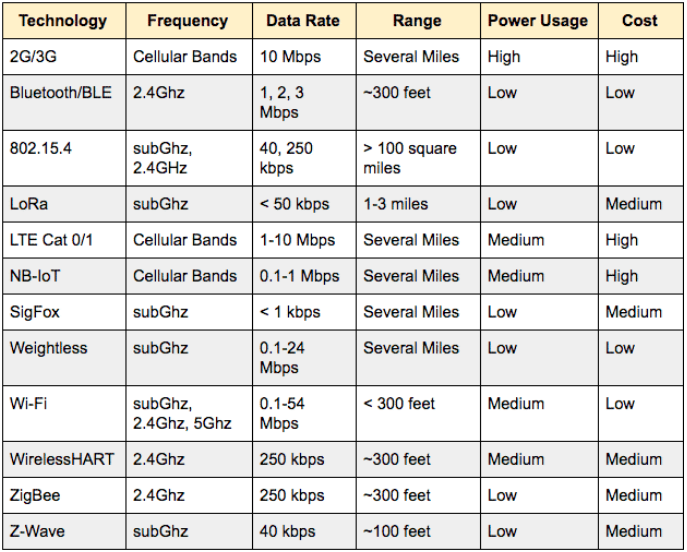
\includegraphics[width=.7\linewidth]{figures/wireless-technologies}
  \caption{Overview of protocols involved in \acrshort{iot} devices and applications \cite{iot-protocols}}
  \label{fig:wireless-technologies}
\end{figure}

\paragraph{Reverse engineering} Reverse engineering is the activity of studying an object to determine its internal function or manufacturing method. It is a common hacking technique since It can be used to understand in detail how a software works, allow bypassing software protections, and ultimately, lead to vulnerabilities. Note that it is common to encounter, when reverse engineering a software, some kind of code obfuscation or anti-debugging measure to prevent it from being easilly reversed.

\paragraph{Hardware hacking} 


\begin{info}
For this work, we essentially apply the penetration testing methodology \acrshort{ptes} to wireless devices, using reverse engineering and hardware hacking to complement the assessment with in depth target understanding.
\end{info}


\section{Tools \& Resources}

In the past, hacking was difficult and required a lot of manual tinkering. Today, hackers have complete suites of automated test tools and processing capabilities that allow them to conduct much more sophisticated attacks, on much larger scales and much faster. In order to end framing the background, various existing security solutions are presented in order to get an overview of what could be usable in the implementation of a penetration test. The remaining of this section presents useful and popular tools distinguished by categories, relevant to penetration testing but not necessarily in our scope. For each tool, it is mentioned if it was used in this project or not.

\subsection{Pentesting platforms}

Two Linux distributions seem to be among the leaders regarding penetration testing ; Kali Linux \cite{kali-linux} and Parrot OS \cite{parrot-os}.

\begin{solutiondata}{kali}
\begin{itemize}[labelsep=1cm]
  \item [\textbf{Type}] Operating System
  \item [\textbf{Purpose}] Reconnaissance, vulnerability analysis, wireless attacks, web application attacks, sniffing and spoofing, reverse engineering, digital forensics, exploit creation, ...
  \item [\textbf{Pros}] Open-source \newline Community supported \newline Various command-line tools
  \item [\textbf{Used}] Yes
\end{itemize}
\end{solutiondata}

{\hyphenation{currently}
\textbf{Kali Linux} \cite{kali-linux} is a Debian-based distribution created by Offensive Security \cite{offensive-security} (another reference in security trainings and certifications) with advanced penetration testing features and tools. This is currently one of the most complete and powerful existing pentesting distributions. It also makes available various command-line tools that are appropriate for scripting and automation. A complete list of the available tools can be consulted at \cite{kali-linux-tools}. One can point out the Metasploit framework \cite{metasploit} as the most interesting and sophisticated tool to perform penetration tests and Volatility \cite{volatility} for digital forensics (essentially the analysis of memory dumps).}

\begin{solutiondata}{parrot}
\begin{itemize}[labelsep=1cm]
  \item [\textbf{Type}] Operating System
  \item [\textbf{Purpose}] Reconnaissance, vulnerability analysis, wireless attacks, web application attacks, sniffing and spoofing, reverse engineering, digital forensics, exploit creation, ...
  \item [\textbf{Pros}] Open-source \newline Lightweight \newline Various command-line tools
  \item [\textbf{Used}] No
\end{itemize}
\end{solutiondata}

\textbf{Parrot OS} \cite{parrot-os} is a free and open source GNU/Linux distribution based on Debian Testing designed for security experts, developers and privacy aware people. Originally developed as part of Frozenbox, the effort has grown to include a community of open source developers, professional security experts, advocates of digital rights, and Linux enthusiasts from all around the globe. It is intended to provide a suite of penetration testing tools to be used for attack mitigation, security research, forensics, and vulnerability assessment.

\subsection{Intelligence Gathering}

As previously evoked, the reconnaissance is the very first of the phases, and it is the one where the pentester will collect the maximum of data on its target before moving on to the following phases. There are a lot of different tools available to the attacker, here are presented a few of the most representative.

\begin{solutiondata}{google}
\begin{itemize}[labelsep=1cm]
  \item [\textbf{Type}] Search Engine
  \item [\textbf{Purpose}] Advanced search on Internet
  \item [\textbf{Pros}] Free \newline Easy to use \newline Finds information that is not readily available on a website
  \item [\textbf{Used}] Yes
\end{itemize}
\end{solutiondata}

\textbf{Google Hacking} \cite{google-hacking} is a technique that relies on the search power of the famous search engine to find accurate information that can help navigate a security breach. To use it, one has to use the Google Dork, they are specific search operators that allow to find accurate data, unlike every day searches, one types keywords in the search bar that can correspond to a text, a title, an image, a meta tag, an alternative text of an image and many others.

\begin{solutiondata}{shodan}
\begin{itemize}[labelsep=1cm]
  \item [\textbf{Type}] Search Engine
  \item [\textbf{Purpose}] Find vulnerable devices
  \item [\textbf{Pros}] Easy to use \newline Indexes all the things connected to the internet
  \item [\textbf{Used}] No
\end{itemize}
\end{solutiondata}

\textbf{Shodan} \cite{shodan} is a website specialized in finding objects connected to the Internet, and therefore having a visible IP address on the network. It allows to find a variety of web servers, routers and many devices such as printers or cameras. Such a request is processed with a simple analysis of the HTTP header returned by the device or server. It is then possible to retrieve lists of specific elements. For each result, it finds the IP address of the server as well as other types of sensitive but accessible information.

\begin{solutiondata}{maltego}
\begin{itemize}[labelsep=1cm]
  \item [\textbf{Type}] Data Mining tool
  \item [\textbf{Purpose}] Providing a library of transforms for discovery of data from open sources, and visualizing that information in a graph format, suitable for link analysis and data mining
  \item [\textbf{Pros}] Highly customizable \newline Graph export options \newline Runs on Windows, Mac and Linux
  \item [\textbf{Used}] No
\end{itemize}
\end{solutiondata}

\textbf{Maltego} \cite{maltego} can be used to determine the relationships between people, websites, documents and files... Connections between these pieces of information are found using open source intelligence (OSINT) techniques by querying sources such as DNS records, Whois records, search engines, social networks, various online APIs and extracting meta data. Maltego provides results in a wide range of graphical layouts that allow for clustering of information which makes seeing relationships instant and accurate – this makes it possible to see hidden connections even if they are three or four degrees of separation apart.

\subsection{Vulnerability Analysis}

New vulnerabilities are emerging every day, within networks, applications, databases. A vulnerability scanner is therefore a computer program designed to assess them for known weaknesses. They are utilized in the identification and detection of vulnerabilities arising from mis-configurations or flawed programming within a network-based asset such as a firewall, router, web server, application server, etc. Modern vulnerability scanners allow for both authenticated and unauthenticated scans. Once again, let’s have a look at some of the most popular ones.

\begin{solutiondata}{nmap}
\begin{itemize}[labelsep=1cm]
  \item [\textbf{Type}] Security Scanner, Port Scanner, Network Exploration Tool
  \item [\textbf{Purpose}] Identifying what devices are running on a network, discovering hosts that are available and the services they offer, finding open ports and detecting security risks
  \item [\textbf{Pros}] Free \newline Well documented \newline Includes many port scanning mechanisms
  \item [\textbf{Used}] Yes
\end{itemize}
\end{solutiondata}

\textbf{Nmap} \cite{nmap} ("Network Mapper") is a free and open source utility for network discovery and security auditing. Nmap uses raw IP packets in novel ways to determine what hosts are available on the network, what services (application name and version) those hosts are offering, what operating systems (and OS versions) they are running, what type of packet filters/firewalls are in use, and dozens of other characteristics. It was designed to rapidly scan large networks, but works fine against single hosts.

\begin{solutiondata}{wireshark}
\begin{itemize}[labelsep=1cm]
  \item [\textbf{Type}] Packet Analyzer
  \item [\textbf{Purpose}] Enables live data reading and analysis for a wide range of network protocols
  \item [\textbf{Pros}] Open Source \newline Display filters are used to filter and organize the data display \newline New protocols can be scrutinized by creating plug-ins
  \item [\textbf{Used}] Yes
\end{itemize}
\end{solutiondata}

\textbf{Wireshark} \cite{wireshark} intercepts traffic and converts that binary traffic into human-readable format. This makes it easy to identify what traffic is crossing a network, how much of it, how frequently, how much latency there is between certain hops, and so forth. While Wireshark supports more than two thousand network protocols, many of them esoteric, uncommon, or old, the modern security professional will find analyzing IP packets to be of most immediate usefulness. The majority of the packets on your network are likely to be TCP, UDP, and ICMP.

\begin{solutiondata}{nessus}
\begin{itemize}[labelsep=1cm]
  \item [\textbf{Type}] Vulnerability Scanner
  \item [\textbf{Purpose}] Identifying what devices are running on a network, discovering hosts that are available and the services they offer, finding open ports and detecting security risks
  \item [\textbf{Pros}] Highly customizable \newline Covers a wide range of technologies \newline Automated reports
  \item [\textbf{Cons}] Full version is expensive
  \item [\textbf{Used}] No
\end{itemize}
\end{solutiondata}

\textbf{Nessus} \cite{Nessus} is a proprietary vulnerability scanner developed by Tenable. Nessus detects live machines on a network, scans open ports, identifies active services, their version, and then attempts various attacks. He then points out the potential or proven weaknesses on the tested machines on a global report. Nessus scans cover a wide range of technologies including operating systems, network devices, hypervisors, databases, web servers, and critical infrastructure. Since version 3, it is licensed, but still free for personal use. Version 2 is maintained. There is also a fork of Nessus 2 still under GPL license called OpenVAS.

\subsection{Exploitation}

With a map of all possible vulnerabilities and entry points, the pentester begins to test the exploits found within your network, applications, and data. The goal is for the ethical hacker is to see exactly how far they can get into your environment, identify high-value targets, and avoid any detection. These actions are once again made easier with the help of multiple tools, some of which are discussed below.

\begin{solutiondata}{metasploit}
\begin{itemize}[labelsep=1cm]
  \item [\textbf{Type}] Penetration Testing Framework
  \item [\textbf{Purpose}] Tool for developing and executing exploit code against a remote target machine
  \item [\textbf{Pros}] Rather intuitive \newline Currently has over 1600 exploits \newline Large user community
  \item [\textbf{Used}] No
\end{itemize}
\end{solutiondata}

\textbf{The Metasploit Framework} \cite{metasploit} is a Ruby-based, modular penetration testing platform that enables to write, test, and execute exploit code. The Metasploit Framework contains a suite of tools that can be used to test security vulnerabilities, enumerate networks, execute attacks, and evade detection. At its core, the Metasploit Framework is a collection of commonly used tools that provide a complete environment for penetration testing and exploit development. More specifically, the MSFconsole provides a command line interface to access and work with the Metasploit Framework. The console lets you do things like scan targets, exploit vulnerabilities, and collect data.

\begin{solutiondata}{john}
\begin{itemize}[labelsep=1cm]
  \item [\textbf{Type}] Offline Password Cracker
  \item [\textbf{Purpose}] Test the security of a password, crack password hashes
  \item [\textbf{Pros}] Open source \newline Extensible (for new crackable hash types) \newline Can leverage graphical card's GPU power for a better performance
  \item [\textbf{Used}] Yes
\end{itemize}
\end{solutiondata}

\textbf{John the Ripper} \cite{john} is a free software for breaking a password, used in particular to test the security of a password. First developed to run under UNIX-derived systems, the program now operates under fifty different platforms, such as BeOS, BSD and its derivatives, DOS, Linux, OpenVMS, Win32. John is one of the most popular password cracking software because it includes the autodetection of hash functions used to store passwords, the implementation of a large number of cracking algorithms, by the fact that it is very easily modifiable, and also that it is possible to resume an attack after a pause.

\begin{solutiondata}{hydra}
\begin{itemize}[labelsep=1cm]
  \item [\textbf{Type}] Online Password Cracker
  \item [\textbf{Purpose}] Test the security of a password, crack passwords on live services
  \item [\textbf{Pros}] Open source \newline Supports a large set of different password hash types \newline Possible to restore a previous aborted/crashed session
  \item [\textbf{Used}] Yes
\end{itemize}
\end{solutiondata}

\textbf{Hydra} \cite{hydra} is a parallelized login cracker which supports numerous protocols to attack. It is very fast and flexible, and new modules are easy to add. Hydra is often John's accomplice. It can take over to break a password online, for example an SSH or FTP, IMAP, IRC, RDP and more. Just point Hydra to the service you want to hack, provide it a list of words, and launch it. Tools like Hydra point out that limiting the password rate and disconnecting users after several unsuccessful login attempts are effective defensive measures against attackers.

\begin{solutiondata}{burp}
\begin{itemize}[labelsep=1cm]
  \item [\textbf{Type}] Web Application Testing
  \item [\textbf{Purpose}] Identify vulnerabilities and verify attack vectors that are affecting web applications
  \item [\textbf{Pros}] Can be used to modify requests to the server, resend them, and observe the results \newline Reported vulnerabilities contain detailed custom advisories
  \item [\textbf{Used}] No
\end{itemize}
\end{solutiondata}

\textbf{Burp Suite} \cite{burp} is a Java based Web Penetration Testing framework. It has become an industry standard suite of tools used by information security professionals. Burp Suite helps you identify vulnerabilities and verify attack vectors that are affecting web applications. In its simplest form, Burp Suite can be classified as an Interception Proxy. While browsing their target application, a penetration tester can configure his internet browser to route traffic through the Burp Suite proxy server. Burp Suite then acts as a (sort of) “Man in The Middle” by capturing and analyzing each request to and from the target web application. Penetration testers can pause, manipulate and replay individual HTTP requests in order to analyze potential parameters or injection points. Injection points can be specified for manual as well as automated fuzzing attacks to discover potentially unintended application behaviors, crashes and error messages.

\begin{solutiondata}{aircrack-ng}
\begin{itemize}[labelsep=1cm]
  \item [\textbf{Type}] WiFi attacks toolkit
  \item [\textbf{Purpose}] Packet sniffing and injection, WEP encryption key recovery
  \item [\textbf{Pros}] Focuses on different areas of WiFi security: monitoring, attacking, testing and cracking \newline All tools are command line which allows for heavy scripting
  \item [\textbf{Used}] Yes
\end{itemize}
\end{solutiondata}

\textbf{Aircrack-ng} \cite{aircrack-ng} is a complete suite of tools to assess WiFi network security. It focuses on different areas of WiFi security :
\begin{itemize}
  \item Monitoring : Packet capture and export of data to text files for further processing by third party tools
  \item Attacking : Replay attacks, deauthentication, fake access points and others via packet injection
  \item Testing : Checking WiFi cards and driver capabilities (capture and injection)
  \item Cracking : WEP and WPA PSK (WPA 1 and 2)
\end{itemize}

\subsection{Reverse engineering}

\textbf{ILSpy}

\textbf{Hopper Disassembler}


\end{chaptercover}

  \insertblankpage
  \begin{chaptercover}{Scope}%
{\coverepigraph{``Drones cause problems for more and more types of secure sites, whether it’s a matter of irresponsible or nefarious operators […] taking photos where you shouldn’t be taking photos or putting people on the ground at risk."}{\textsc{Nimo Shkedy} \newline {\normalsize\vspace{-.3cm}CEO of ApolloShield}}
{\large \hyphenation{} \bigletter{}{} {\color{red} ...}\newline\\}}%
{scope}

Now that we have set the basics of what is penetration testing, we can move to the actual application of the concept to the drones. 

The first phase of the work consists in gathering as much information as possible regarding the current state-of-the-art on drone security.

\section{Literature review}

This section focuses on showing a possible design of a drone and a compilation of security-relevant information. As part of that effort, the following emphasizes on giving a ready reference of one particular vulnerable drone and associated open source attack tools that have already been developed. This compilation should provide the reader with a better understanding of how drone vulnerability is currently exploited, and how future drone will take advantage of improvements in available vulnerability research data.

\subsection{Typical drone design}



\subsection{Parrot AR Drone}

\begin{center}
\begin{tabular}{m{5cm}m{12.3cm}}
\hyphenation{produced}
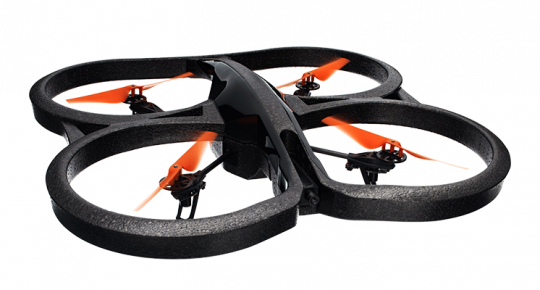
\includegraphics[width=\linewidth]{parrot-ar-drone-2} & The Parrot AR Drone 2.0 is one of the most popular quadcopters produced. This is a cheap drone that is both quick and fast. It is controlled by an iOS or Android smartphone or tablet and allows 720p live high-definition video streaming and recording in flight. \\
\end{tabular}
\end{center}

This device is a good reference on how one of the most popular commercial drones totally lacks security. Security breaches are numerous, let’s review them :
\begin{itemize}
  \item \textbf{Open FTP on port TCP/21} : Simply just connect to the IP without any username or password, and have access to the directory of the drone, where it stores the recorded videos.
  \item \textbf{Open Telnet on port 23} : Once again, simply just connect to the IP without any username or password, and you are logged in. Furthermore, it's running Linux and it is a root access to the device! At this point the attacker could simply issue a shutdown and watch the drone fall to the ground.
  \item \textbf{Unencrypted communications} : A simple capture of the communication packets between the drone and the controller allows the attacker to have an easy view of the protocol. Once he has successfully analyzed the main commands, he can easily replay them -- for example using the python Scapy library -- in order to hijack the drone.
  \item \textbf{WiFi controlled} : The drone is controlled with an app through WiFi, and by default, it isn’t even password-protected ! This allows any user running the application to control the drone. Even though a security can be enabled, called \textit{Pairing}, which will make the drone drop the packets if the MAC address sending them is not the one it is paired with. It is nonetheless easy for the attacker to spoof the source MAC on the packets.
\end{itemize}

More information can be found on the subject at \cite{github-drone-hacking} as well as some investigations for improving the security at \cite{hacking-securing-ardrone2}.

\subsection{Known vulnerabilities}

As defined in Subsection \ref{subsec:vuln-vs-weakness}, \acrshort{cve}'s are identifiers for publicly known vulnerabilities. It is therefore useful, prior to starting any pentest on drones, to look for eventual known vulnerabilities on the field. In the same way, CVE may be used once a certain service is identified on a device.

As for now, only one entry is available and concerns the DBPOWER U818A WIFI quadcopter drone :
\begin{itemize}
  \item \textbf{CVE-2017-3209} : \textit{The quadcopter drone provides \textbf{FTP} access over its own local access point, and allows full file permissions to the anonymous user. The DBPower U818A WIFI quadcopter drone runs an FTP server that by default \textbf{allows anonymous access without a password}, and provides full filesystem read/write permissions to the anonymous user. A remote user within range of the open access point on the drone may utilize the anonymous user of the FTP server to read arbitrary files, such as images and video recorded by the device, or to replace system files such as /etc/shadow to gain further access to the device. Furthermore, the DBPOWER U818A WIFI quadcopter drone uses BusyBox 1.20.2, which was released in 2012, and may be vulnerable to other known BusyBox vulnerabilities.}
\end{itemize}

It goes without saying that a single result is terribly weak, for example, we get nearly 1,500 results just for the Apache web server (as August 2019). This tends to show that a substantive work remains to be done in this area, but also that the door is open for real progress.

{\color{red}
Here insert a note on some commercial projects such as:
\begin{itemize}
  \item ApolloShield:  https://www.apolloshield.com/
  \item Talk about the many “non-hacking” solutions
\end{itemize}}

\section{Scope definition}

This section presents some models of drones selected for the study and the beginning of the application of the penetration testing methodology, that is, the \textit{intelligence gathering}.

\subsection{Scope limitation}

The drones were provided by the professional supervisor within the limits of his allocated budget to cover a small spectrum of drone-related technologies in order to establish the basis of a framework (as it is explained in Chapter \ref{framework}). For a question of scope, only a few models are selected to match some technical specifications as we focus on wireless penetration testing.

For this work, we received the following six different drones. Each of them comes from a different brand so that we can cover the wider spectrum of technologies possible.
\begin{itemize}
  \item Drone S9
  \item Jamara Skip 3D Quadrocopter
  \item NINCOAIR QUADRONE MINI
  \item UdiR/C Free Loop U27 
  \item Flitt Selfie Cam
  \item C-me 1080P WiFi FPV GPS Selfie Drone
\end{itemize}

In the initial problem statement, it was decided to develop plugins for at least 3 different popular commercial drones on the framework according to the exploits that could be discovered. Rather quickly, we excluded the first four since they were not WiFi- but radio-controlled and should require the use of a different technology than the one aimed in this work. It leaved us with the last two.

\subsection{Flitt Selfie Cam}

\begin{center}
\begin{tabular}{m{5cm}m{12.3cm}}
\hyphenation{produced}
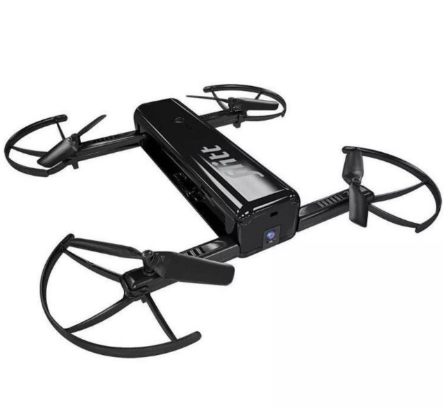
\includegraphics[width=\linewidth]{figures/flitt-selfie-cam} & \textit{Flitt Flying Camera is a pocket-sized flyer that features an adjustable CMOS camera that can record 720p video at 30 fps and shoot 1.3MP photos. The Flitt uses 2.4 GHz Wi-Fi to communicate with either an Android or IOS free companion app. From the app, you can fly the Flitt, take pictures and video, adjust camera pitch, change the photo mode, and more.} \\
\end{tabular}
\end{center}

\begin{figure}[H]
  \centering
  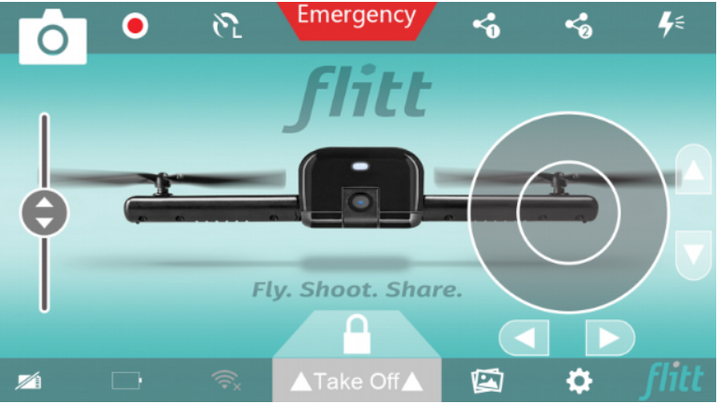
\includegraphics[width=0.7\linewidth]{figures/flitt-selfie-cam-ui}
  \caption{User interface for piloting the Flitt Selfie Cam from a smartphone}
  \label{fig:flitt-selfie-cam}
\end{figure}

The device must be unlocked in order to take off, auto-regulates its high and has an emergency landing feature in case of loss of control.

\subsection{C-me Selfie Drone}

\begin{center}
\begin{tabular}{m{5cm}m{12.3cm}}
\hyphenation{produced}
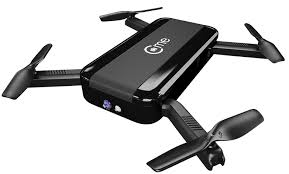
\includegraphics[width=\linewidth]{figures/cme-selfie-drone} & \textit{C-me flying camera is designed to be the ultimate flying "selfie stick" for capturing life’s memorable events thanks to its 8MP HD 1080p camera. It comes with an intuitive app control that interfaces with iOS and most Android phones and tablets. It communicates through 2.4 GHz Wi-Fi. Its size allows to easily fit in a pocket, purse or backpack.} \\
\end{tabular}
\end{center}

\begin{figure}[H]
  \centering
  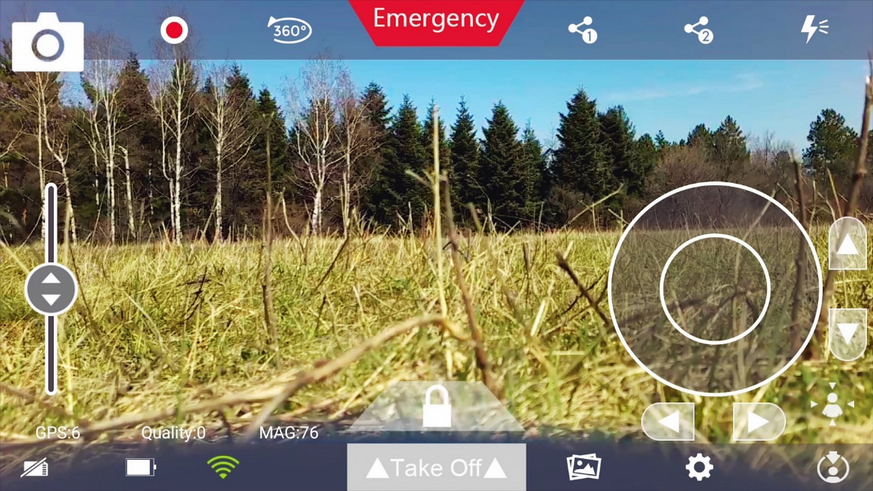
\includegraphics[width=0.7\linewidth]{figures/cme-selfie-drone-ui}
  \caption{User interface for piloting the C-me Selfie Drone from a smartphone}
  \label{fig:flitt-selfie-cam}
\end{figure}

Once again, the device must be unlocked in order to take off, auto-regulates its high and has an emergency landing feature in case of loss of control.

\begin{tip}
It is quite obvious that the interfaces are quite similar, and after further research, it turns out that the two drones are produced by the same manufacturer, i.e. Hobbico. This means that there will probably be similarities between the two devices, even though the C-me has more functionalities since it’s a little bit more expensive than the Flitt (depending on the reseller, in the 150\euro range versus 80\euro). This will be a good occasion to compare them and see if one is more secure than the other.

Hobbico, Inc. was a manufacturer and distributor of hobby products including radio control airplanes, boats, cars, helicopters and drones. Unfortunately, on 2018, it was announced that Hobbico had filed for Chapter 7 bankruptcy and went into liquidation1, and the company was later bought by Horizon Hobby2. There website, hobbico.com, is no longer available online and there is no reference to any of the drones on the Horizon Hobby website meaning that there is no support anymore for them.
\end{tip}

\subsection{Intelligence gathering}


\section{Vulnerability analysis}


\end{chaptercover}

  \insertblankpage
  \begin{chaptercover}{Exploits}%
{\coverepigraph{``I get hired by companies to hack into their systems and break into their physical facilities to find security holes. Our success rate is 100\%; we've always found a hole."}{\textsc{Kevin Mitnick} \newline {\normalsize\vspace{-.3cm}Cybersecurity consultant}}
{\large \hyphenation{} \bigletter{S}{ystems} have almost always flaws. No \acrshort{is} should ever be considered as completely secure. Even if everything seems to be perfectly hermetic to an attacker, it is always a matter of time before a vulnerability is discovered and the system could be breached. \newline \\ In this chapter, we will put to use the findings discovered in Chapter \ref{scope} in order to exploit the drones in ways unintended by the manufacturer. \newline\\}}%
{exploits}

Now that we have performed our vulnerability analysis, we have a better understanding of how both drones operate. Strong with this knowledge, we will try to gain access or control of them in ways not intended by the manufacturer.

\lstset{
  language=bash,
  backgroundcolor=\color{lightgray},
  showstringspaces=false,
  basicstyle=\ttfamily\color{black},
  commentstyle=\ttfamily\color{black},
  keywordstyle=\ttfamily\color{blue}
}

\section{Flitt Selfie Cam}

This section details a few successful exploits that could be achieved.

\subsection{Telnet attack}

The first possible weakness of the device is the open port TCP/23 allowing telnet connection. Unfortunately, there were no feature in the app that uses the functionality so we were not able to intercept the password nor find it in the code of the APK.

We the decided to give a go to a dictionary attack. It involves testing a series of potential passwords, one after the other, hoping that the password used for encryption is contained in the dictionary. To that end, the first step is to get ourselves a good dictionary. As already presented in Subsection \ref{subsec:hacking-techniques}, the RockYou wordlist is certainly a good choice in terms of completeness as it contains more than 14 million unique passwords and it is shipped with Kali Linux, the distribution we use.

Next is to set up a dictionary attack on a telnet service. To achieve that, we used the Hydra tool (presented in Subsection \ref{subsec:tools-and-resources}). It is fairly simple to use, using the following syntax :

\begin{center}
\begin{minipage}{.95\linewidth}
\begin{lstlisting}
root@kali:~# hydra -l <username> -P <password_file> telnet://targetname
\end{lstlisting}
\end{minipage}
\end{center}

We were confronted to two main issues :
\begin{enumerate}
  \item We had no idea which username is allowed to use the telnet service on the drone side. By default, we tried it with the \texttt{root} account.
  \item The battery of the drone has to be removed in order to be charged and only last for around one hour. It is relatively slow to establish a telnet connection, since it is TCP based, and we were only able to test around 10.000 password each hour before having to pause the attack and recharge the battery.
\end{enumerate}

We proceeded with the attack until we tested around 100.000 passwords, but the odds of a success were considered to low considering the two issues above so we decided to move on.

\subsection{\acrshort{uart} shell access}

This process started with physically opening the device in order to determine the precise hardware in use. Through manual inspection of the device’s internals, it was possible to obtain the relevant component datasheets from the Internet. The chip used in the Flitt Selfie Cam is a Hi3518 \cite{hi3518-datasheet}, which is designed for light video processing, and mostly used in IP cameras. 

Two of the most common relevant interfaces for hardware hacking are \acrfull{uart} and \acrfull{jtag}. \acrshort{jtag} is immensely powerful, usually providing read and write from memory, debugging, extract Firmware, bypass protection mechanisms and more. However, it can be rather difficult to use and requires additional hardware. \acrshort{uart}, on the other hand, is much less powerful but much easier to work with, and usually only uses 2-3 pins (ground, TX and RX). Fortunately, on a lot of IoT devices, an exposed \acrshort{uart} interface is almost always used by the bootloader and OS for a hardware console.

The next step is going to be to identify the different pins that are responsible for the \acrshort{uart} communication. As can be seen on the datasheets, the Hi3518 has 3 sets of \acrshort{uart} pins like presented in Appendix \ref{app:uart-pins}. Our goal here would be to connect to the \acrshort{uart} 0 pins in order to obtain a shell access.

\begin{figure}[H]
\begin{center}
\begin{tabular}{m{9.5cm}m{7.8cm}}
  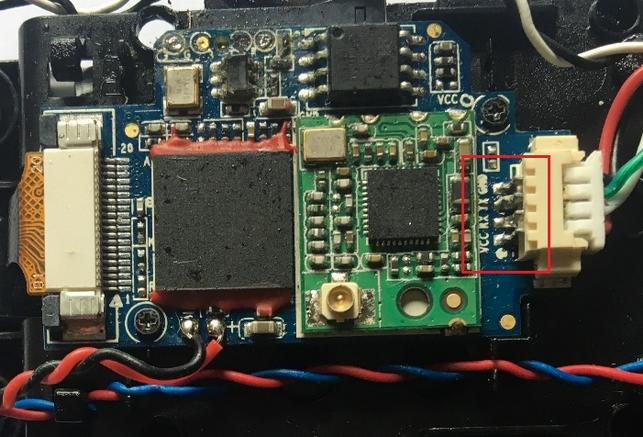
\includegraphics[width=\linewidth]{uart-pins}
  \caption{Bad set of \acrshort{uart} pins of the Flitt Selfie Cam}
  & We could identify a first set of pins rather quickly and proceeded to solder wires on the TX, RX and ground respective pins. Notice that the pins connect to a cable which leads to a second PCB responsible for the control of the 4 motors. It is therefore likely that there are the \acrshort{uart} 1 pins. \\
\end{tabular}
\end{center}
\end{figure}

The procedure was tested using the standard baud rates for serial devices, being 110, 300, 600, 1200, 2400, 4800, 9600, 14400, 19200, 38400, 57600, 115200, 128000 and 256000 bits per second \cite{baudrate}. As it can be seen in Figure \ref{fig:uart-shell-access-failure}, the connection was not successful. 

\begin{figure}[H]
  \centering
  
\includegraphics[width=.8\linewidth]{figures/uart-shell-access-failure}
  \caption{Failure in getting shell access through the \acrshort{uart}}
  \label{fig:uart-shell-access-failure}
\end{figure}

But as much as these first tests were not successful, they at least demonstrated that some communication was happening, which was rather encouraging.

\begin{figure}[H]
\begin{center}
\begin{tabular}{m{8cm}m{9.3cm}}
  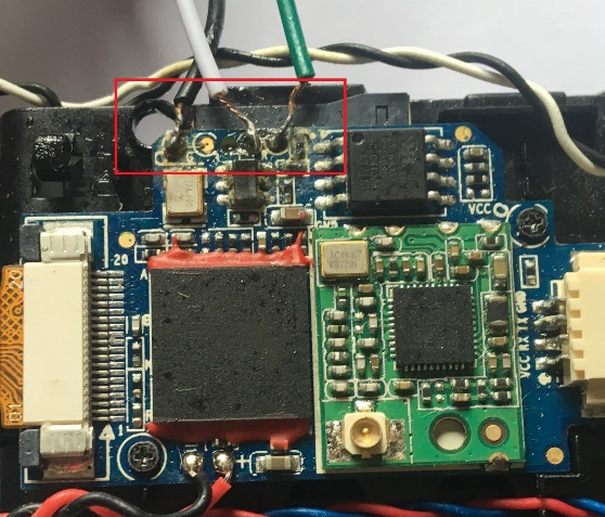
\includegraphics[width=\linewidth]{uart-pins-2}
  \caption{Good set of \acrshort{uart} pins of the Flitt Selfie Cam}
  & There were fortunately four more pins, with G, T and R tags on the side to which nothing seemed to be connected. I made sure that the G tagged pin was indeed the ground by checking the continuity between it and a known ground point on the drone with a multimeter. I then soldered my wires, connected the serial cables (Rx from the computer-side with Tx, and vice-versa). The console port of the card turns out to use a baud rate of 115,200 bauds, 8-bit data, no parity and a stop bit (abbreviated as 115200 8N1), as shown in Figure \ref{fig:uart-putty-session} when using PuTTY on Windows. Hardware flow control must be disabled. \\
\end{tabular}
\end{center}
\end{figure}

\begin{figure}[H]
  \centering
  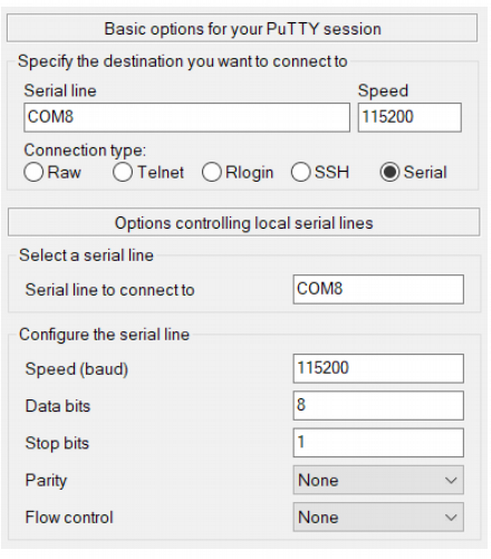
\includegraphics[width=.5\linewidth]{uart-putty-session}
  \caption{PuTTY parameters for opening a session through the \acrshort{uart}}
  \label{fig:uart-putty-session}
\end{figure}

Finally, when the connection to the serial port via \acrshort{uart} is established. A Linux-based startup sequences is displayed and, and we automatically have a root shell access to the drone !

\begin{figure}[H]
  \centering
  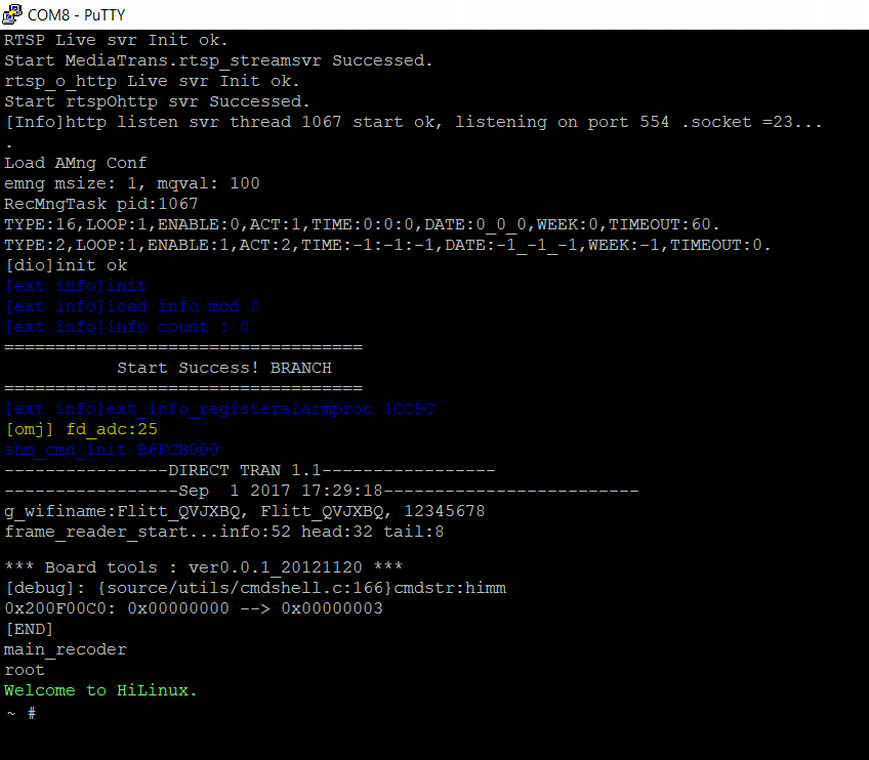
\includegraphics[width=\linewidth]{uart-shell-access-success}
  \caption{Success in getting shell access through the \acrshort{uart} on the Flitt}
  \label{fig:uart-shell-access-success}
\end{figure}

Having a shell available, it was easy to easy to recover the hash of the root password in the \texttt{/etc/passwd} file : 

\begin{center}
\begin{minipage}{.95\linewidth}
\begin{lstlisting}
root:$1$dfU0W8J6$vKtbAXdyZmq5GbYveqnnJ.:0:0::/root:/bin/sh
\end{lstlisting}
\end{minipage}
\end{center}

After analyzing the hash with the hash-identifier tool from Kali Linux, we were able to identify it as being a MD5, as shown in Figure \ref{fig:hash-identifier-root}.

\begin{figure}[H]
  \centering
  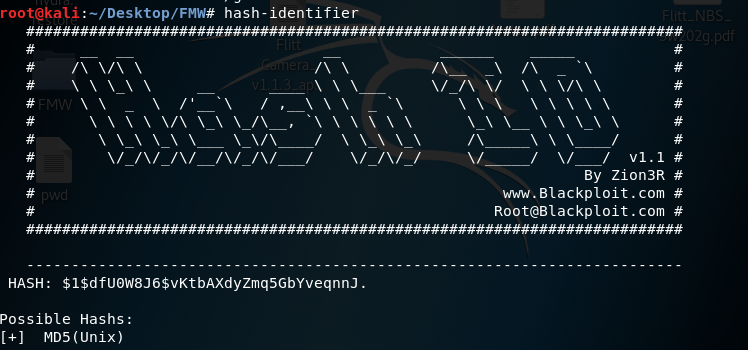
\includegraphics[width=.75\linewidth]{hash-identifier-root}
  \caption{Identifying the root password has as a MD5}
  \label{fig:hash-identifier-root}
\end{figure}

Finally, with the help of Johnny (a graphical version of the cracking program John the Ripper), and the \texttt{rockyou.txt} dictionary, we were able to crack the hash in a few minutes and therefore obtain the root password : \textbf{\texttt{ev1324}} (as shown in Figure \ref{fig:johnny-root-password}).

\begin{figure}[H]
  \centering
  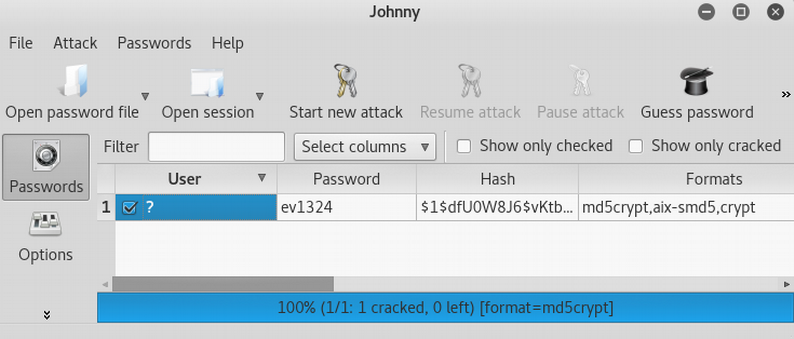
\includegraphics[width=.85\linewidth]{johnny-root-password}
  \caption{Recovering the root password}
  \label{fig:johnny-root-password}
\end{figure}

The password allowed to successfully connect to the drone with telnet, it was therefore not necessary anymore to access through the serial method.

\begin{tip}
As can be seen here, the password is the 8240422\textsuperscript{th} on the Rockyou list. It would therefore have taken roughly 34 days and 8 hours before we could successfully carry out the Telnet dictionary attack. And this is considering that we were lucky enough to guess the right user being root.

\begin{center}

\includegraphics[width=.5\linewidth]{figures/rockyou-root-password}
\end{center}
\end{tip}

\section{C-me Selfie Drone}

This section details a few successful exploits that could be achieved.

\subsection{\acrshort{uart} shell access}

Strong with the knowledge acquired on the Flitt Selfie Cam, we applied the same technique to the C-me Selfie Drone.

\begin{figure}[H]
\begin{center}
\begin{tabular}{m{9cm}m{8.3cm}}
  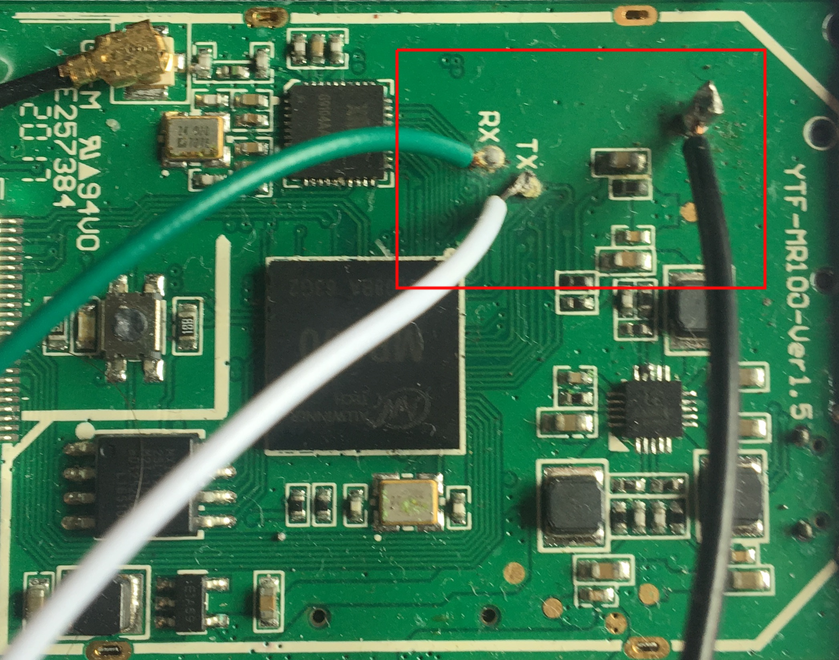
\includegraphics[width=\linewidth]{uart-rx-tx-pins}
  \caption{Set of \acrshort{uart} pins of the C-me Selfie Drone}
  & After opening the device, we quickly noticed unused connectors tagged with Rx and Tx. Therefore, it only remained to find a Ground spot using a multimeter and to proceed soldering the wires. \\
\end{tabular}
\end{center}
\end{figure}

\vspace{-1cm}
And using once again the same process, trough putty and a serial connection, we could obtain a root shell on the drone.

\begin{figure}[H]
  \centering
  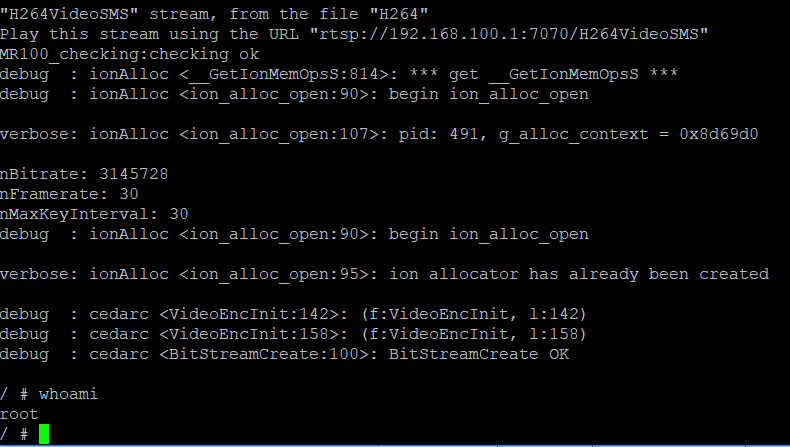
\includegraphics[width=.95\linewidth]{uart-shell-access-success-2}
  \caption{Success in getting shell access through the \acrshort{uart} on the C-me}
  \label{fig:uart-shell-access-success-2}
\end{figure}

The goal of the procedure was to gather information on the firmware from the device so that it could be reverse engineered in order to identify the services running and software vulnerabilities. Additionally, the activation of a remote management service was desirable in order to provide elevated privileges to the end-user, but couldn’t be done in an easy way since the filesystem was writing protected. This will be developed in the post-exploitation section.

\subsection{Sending config commands}\label{subsec:sending-config-commands}

Using the same procedure as in Subsection \ref{subsec:reverse-engineering}, we proceeded to change some drone's configuration, such as the WiFi password, and capture the resulting packets.

By analyzing the packets, we were able to establish that those commands are sent to the port TCP/4646, and have the syntax as shown on Figure \ref{fig:config-command}.

\begin{figure}[H]
  \centering
  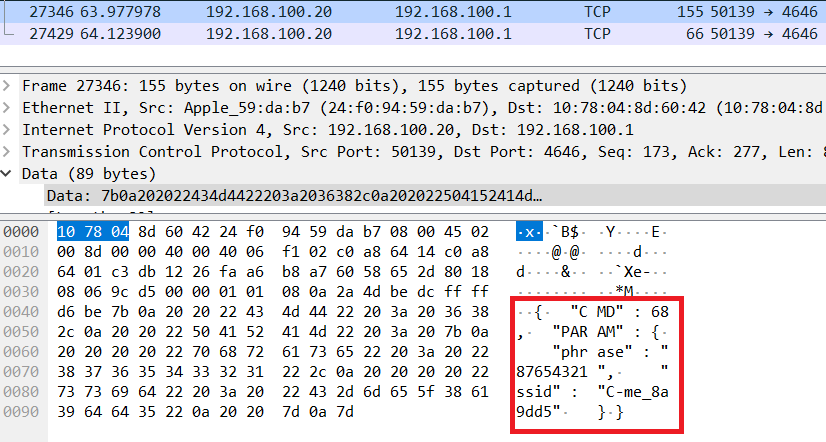
\includegraphics[width=\linewidth]{figures/config-command}
  \caption{Result of a configuration command viewed in Wireshark}
  \label{fig:config-command}
\end{figure}

And logically, we could identify the \texttt{CMD\_REQ\_NET\_PASSWORD} being the 69\textsuperscript{th} element of the enumeration discovered earlier in the config file present within the code of the APK. From here, we should be able to forge some equivalent packets in order to hack the drone.

\subsection{Post-exploitation}\label{subsec:post-exploitation}

Not being able to write on the C-me filesystem was problematic, as we felt close to our goal, getting persistent access to a shell from a distance.

Fortunately, the drone had a firmware update feature that is triggered from the smartphone application. Moreover, the only two directories that could be written on the device were obviously the \texttt{/mnt}, on which was mounted the SD card, but also a directory name \texttt{/netPrivate}. After investigation, the \texttt{/netPrivate} folder contained a specific file, named \texttt{config.dat}, that only consisted in a list of values, seeming to match the drone’s current configuration. 

Having done the update of the firmware previously without much notice, the drone was up-to-date (at version 0.7.15). It was thus no longer possible to trigger an update from the smartphone, and then to capture the traffic exchanged in order to reverse the update process.

Conveniently, in the list of values found in the \texttt{config.dat} file, one of the values matched "\texttt{0.7.15}", and since it was possible to write in the file, we proceeded to change the value to "\texttt{0.7.14}" to see if it made any difference. It did ! We were once again prompted with a message on the smartphone asking if we wanted to do a firmware update (even though the firmware was already up-to-date on the drone, we thus simply tricked the system into believing that it was not). This allowed us to capture the packets exchanged while a firmware update was happening, the same way as detailed in Subsection \ref{subsec:traffic-analysis}.

By studying the packets in Wireshark, and searching for the FTP protocol, we were able to use the functionality "\textit{follow the TCP stream}" and to uncover the whole sequence of FTP commands necessary to send a new firmware to the drone, as depicted in Figure \ref{fig:ftp-tcp-stream}. Then together with a specific control command (identification number 71) as shown in Figure \ref{fig:config-command}, we could trigger the update of drone's OS.

\begin{figure}[H]
  \centering
  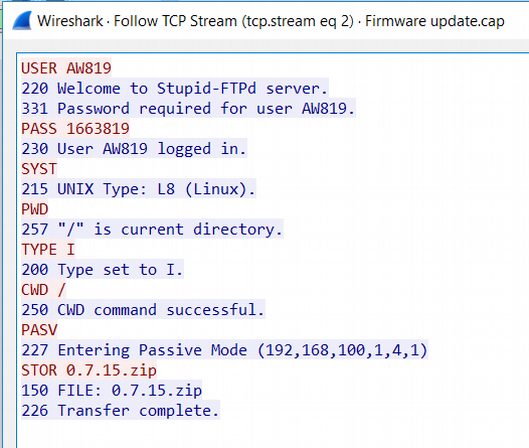
\includegraphics[width=.6\linewidth]{figures/ftp-tcp-stream}
  \caption{TCP stream of an FTP update transfer session on the C-me Selfie Drone}
  \label{fig:ftp-tcp-stream}
\end{figure}

We could also recover the \texttt{0.7.15.zip} file containing the firmware. From this point, we were now able to update the firmware of the drone from our computers.

Inside the archive, a file named \texttt{rootfs.squashfs} was present. SquashFS \cite{squashfs} is an open source, read only, extremely compressible filesystem. The SquashFS filesystem tools come in a separate package. This package is called \texttt{squashfs-tools} \cite{squashfs-tools}. Once installed, it is possible to open the file and inside can be found the entire filesystem of the C-me drone !

At this point, we were able to locate a script in \texttt{/etc} named \texttt{autorun.sh} that is used to launch a set of services at boot time. We thus simply added a line having the effect of launching the Telnet service and re-created the archive.

Once the new modified firmware was uploaded, the telnet service was running on the drone from the boot and we could connect to it with the root user via Telnet. We now have created a backdoor on the device !

\begin{summary}
The \textbf{exploitation} is probably the \textbf{most rewarding step} of all the pentesting process. Indeed, this is the moment when the attacker put to the test the vulnerabilities found in the previous phases to advance in the intrusion of the information system. Obviously, the outcome of the exploitation phase is highly dependent on the quality of the research already achieved.

\textbf{Two} different \textbf{scenarios} are possible at this stage :
\begin{itemize}
  \item Either you have uncovered an already \textbf{known vulnerability} that can be \textbf{exploited with a tool} or an attack that is usable with few efforts.
  \item Either there is a vulnerability, but it is up to the attacker to \textbf{come with an innovative solution} that can either be a piece of code or a clever use of an existing tool.
\end{itemize}

During the process of our exploitation phase we were brought to put into direct practice the latest statement. Indeed, \textbf{some exploits were} rather \textbf{straightforward}, with many examples in the literature and therefore consisted more in a technical execution, but some others had to be forged by us.

In short, on the \textbf{Flitt Selfie Cam} we carried out a dictionary attack in an attempt to crack the telnet credentials. Being unsuccessful, we opted to open the device and perform a hardware hacking of the \acrshort{uart} serial line. This resulted in obtaining a \textbf{root shell} access to the OS. From within, it was therefore possible to crack the root account’s password through its hash. Once the \textbf{password uncovered}, we had direct access on the drone thanks to the \textbf{Telnet} service.

On the \textbf{C-me Selfie Drone}, we first tried to exploit the FTP service without any luck. Then, strong with the hardware hack knowledge and success gained on the Flitt, we applied once again the same procedure with the \textbf{same outcome} on the C-me. Once inside, we could establish that a Telnet service was indeed installed on the drone but not running by default. Unfortunately, impossible to write anything on the filesystem except for the \texttt{/mnt} repository, as it was protected.

Finally, on \textbf{both drones}, we were able to \textbf{forge configuration commands}, through python scripts, that allowed us to change critical information on the drones, such as the \acrshort{ssid} or the WiFi password ; as well as deleting the video media or even shutting it down.

Not giving up on the \textbf{C-me Selfie Drone}, we managed to understand how the \textbf{firmware update} process was working and were able to forge our own firmware in which the telnet service was activated. Once updated, the drone therefore contained a \textbf{backdoor} that we could then exploit a our advantage, thus adding a post-exploitation component to our whole process.
\end{summary}

\begin{discussion}
Once the reconnaissance and vulnerability analysis phases are completed, the pentester should have a more thorough understanding of his target. At this point, a list of weaknesses and possible attack vectors allows him to plan which attack has the higher chances to succeed.

In our process, we naturally focused first on attacks that were involving automated tools to be carried out. For instance, a dictionary attack on the telnet server of the Flitt or some tries to make usage of some Metasploit’s built in exploits on the FTP server of the C-me or directly on the Linux OS of the drones.

But after as many failures as there were attempts, the hope of success was shrinking quickly and one could ask if we were really up to the task.

Later, by checking know hacks in the scope of the Hi3518 chip (which is the main chip of the Flitt and is commonly used on light video devices), we stumbled upon a methodology allowing to obtain root shell access on an IP camera that was base on the same chip. Though it was some hardware hacking.

Initially, we didn’t consider hardware hacking as part of the scope of the work, but having no better alternative at this point we decided to apply the described methodology to the drone. 
In order to perform this hack, the attacker has to physically connect wires to an UART serial line eventually left unprotected by the manufacturer. We would like to express our gratitude to Ir Valéry Broun for devoting his precious time to the soldering of the necessary wires.

The hack didn’t succeed on the first try, notably because there were more than one serial line on the PCB, but after a week of trying and a steep soldering learning curve, we finally managed to obtain a shell access to the drone’s OS.

Strong with the former experience, the hack was quickly repeated on the C-me drone, following the exact same methodology. We might have uncovered a pattern to hack light video drones
From this point, we were able to dig into the OS of both devices, and finally take full advantage of all the information gathered during the reconnaissance and vulnerability analysis phases.

As Kevin Mitnick stated, there is always a hole to break into a system. We learned from this experience that the key to success is, after knowledge, perseverance.
\end{discussion}

\end{chaptercover}

  \insertblankpage
  \begin{chaptercover}{Framework}%
{\coverepigraph{``Any program is only as good as it is useful."}{\textsc{Linus Torvalds} \newline {\normalsize\vspace{-.3cm}Creator of Linux}}
{\large \hyphenation{} \bigletter{F}{rameworks} are flourishing these days, especially in cybersecurity (e.g. Metasploit \cite{metasploit}). These kinds of toolkit generally gather a lot of knowledge acquired and automated by a myriad of security experts, trying to provide a solution as complete as possible. \newline \\ DroneSploit, the framework we propose to build, is an attempt to mechanize drone hacking techniques in particular, the most user-friendly way possible. This chapter presents the basics of its underlying library and the exploits we could automate in the new framework. \newline\\}}%
{framework}

\lstset{
language=python,
basicstyle=\ttfamily,
%otherkeywords={self},             % Add keywords here
keywordstyle=\ttfamily\color{SecondBlue},
%emph={MyClass,__init__},          % Custom highlighting
emphstyle=\ttfamily\color{venetianred},    % Custom highlighting style
stringstyle=\ttfamily\color{forestgreen(web)},
commentstyle=\ttfamily\color{prune},
frame=tb,                         % Any extra options here
showstringspaces=false            % 
}

\section{Sploitkit}

This section succinctly presents Sploitkit, a \textit{toolkit for building Metasploit-like consoles}. \cite{sploitkit}

\subsection{Philosophy}

\textit{Sploitkit is a framework designed to quickly build CLI consoles with a style ressembling that of Metasploit. It features a clear and intuitive plugin architecture that allows to build consoles with new commands or modules but also models for their internal stores. This is another framework made according to the \acrshort{dry} philosophy.} \cite{sploitkit-docs}

Briefly, this framework written in Python is built to facilitate the creation of new penetration testing consoles tailored to specific use cases, especially when these are not extensively covered in some well-known frameworks like Metasploit. It uses a popular Python3-only package called \texttt{prompt\_toolkit} \cite{prompt-toolkit} designed to make beautiful CLI applications with, for instance, dropdown lists (for command autocompletion), menus or toolbars.

\subsection{\acrlong{api}}

Sploitkit aims to provide an easy and convenient \acrshort{api} for quickly extending the console with new commands, modules and store models in an object oriented manner. It defines multiple \textit{entities} which are customizable by the developer :
\begin{itemize}
  \item \texttt{Console} : This is the class used to define new (sub)console levels. As it suggests, a level (defined with the \texttt{level} attribute) will determine a scope for the related console, allowing to filter out unapplicable entities (like commands and modules). Its prompt (added to its parent's level) can be customized with the \texttt{prompt} attribute.
  \item \texttt{Command} : This class allows to define a command callable from a console through the definition of its \texttt{run()} method. When bound to a console, it has an attribute with the same name to be able to use console's configuration settings. A command can be associated with a console level or with every level except those defined in the \texttt{except\_levels} attribute. It can also have aliases (using the attribute with the same name). Also worth being mentioned, a command can define completion methods (\texttt{complete\_values} and \texttt{complete\_options}) and/or a \texttt{validate} method to fine-tune its working and feedback to the user.
  \item \texttt{Module} : This class allows to gather complex computation aimed to run inside a dedicated console level, just like Metasploit and other ressembling frameworks do (typically selecting a module with a \texttt{use} command, then setting module's parameters before running the \texttt{run} or \texttt{exploit} command). This logic is defined in the \texttt{run()} method.
  \item \texttt{BaseModel}, \texttt{Model}, \texttt{StoreExtension} : These classes aim to refine data store's structure with new \acrshort{orm} models. Typically, new models will be defined subclassing \texttt{Model} while \texttt{BaseModel} will be used for association tables. The \texttt{StoreExtension}'s allow to add custom methods to the store by behaving like mixin classes included in store's class inheritance.
\end{itemize}

With these entities, all the mechanics of a good console can easilly be declared to create a new CLI framework dedicated to ones use case. For more details on how to use the different \acrshort{api}'s, the interested reader can refer to Sploitkit's documentation \cite{sploitkit-docs}.

\subsection{Quick start}\label{subsec:sploitkit-quickstart}

The following demonstrates Sploitkit's easy and comprehensive interface to quickly get started :

\paragraph{Start with a \texttt{FrameworkConsole}} A main file can be created to put the subclassed \texttt{FrameworkConsole} as a basis for the new console, as shown below.

\begin{center}
\begin{lstlisting}[caption={Main file \texttt{main.py} for the new console},emph={MySploitConsole,FrameworkConsole}]
#!/usr/bin/python3
from sploitkit import FrameworkConsole

class MySploitConsole(FrameworkConsole):
    # set your console items here
    pass
    # default sources:
    #sources = {
    #    'banners':  None,
    #    'entities': ["commands", "models", "modules"],
    #} 

if __name__ == '__main__':
    MySploitConsole(
        "MySploit",
        # configure your console settings here
    ).start()
\end{lstlisting}\label{lst:framework-console}
\end{center}

As mentioned in the comments in Listing \ref{lst:framework-console}, some default sources are defined. These are the base folders where Sploitkit will search for additionnal commands, modules and models. Accessorily, Sploitkit provides a funny feature allowing to generate banners from the application name (here "\texttt{MySploit}") and converting images from the \texttt{banners} source folder (i.e. in JPG or PNG format) to ASCII images for display at console's startup.

\paragraph{Adding a \texttt{Command}} Commands can be created in separate files, saved in one of the folders from sources' \texttt{entities} field. An example of command is shown hereafter. This is a command included in the base entities of Sploitkit.

\begin{center}
\begin{lstlisting}[caption={Commands file \texttt{sploitkit/base/module.py} from Sploitkit},emph={Use,Command,run}]
# -*- coding: UTF-8 -*-
from sploitkit import *
[...]
class Use(Command):
    """ Select a module """
    def complete_values(self):
        return Module.get_list()
    
    def run(self, module):
        new_mod, old_mod = Module.get_modules(module), self.module
        # avoid starting a new subconsole for the same module
        if old_mod is not None and old_mod.fullpath == new_mod.fullpath:
            return
        ModuleConsole(self.console, new_mod).start()
[...]
\end{lstlisting}\label{lst:framework-command}
\end{center}

This is an example of a command starting a subconsole. It uses the list of loaded modules for value autocompletion. Note that Sploitkit handles the validation by itself using the return value of \texttt{complete\_values}, this prevents the developer from rewriting code handling the same list of values.

\paragraph{Adding a first \texttt{Module}} A module can be created by simply subclassing \texttt{Module}, defining its custom configuration and its \texttt{run()} method like shown in Listing \ref{lst:framework-module}.

\begin{center}
\begin{lstlisting}[caption={Module file \texttt{my-first-module.py}},emph={MyFirstModule,Module,run,config,Config,Option}]
# -*- coding: UTF-8 -*-
from sploitkit import Config, Module, Option

class MyFirstModule(Module):
    config = Config({
        Option("PARAM", "param description", True): "default_value",
    })
    path = "path/to/module"  # module will be called with
                             # 'path/to/module/my_first_module'
    def run(self):
        # do something
        pass
\end{lstlisting}\label{lst:framework-module}
\end{center}

Module's path (for calling it with the \texttt{use} command from a console) can be defined in two different ways :
\begin{enumerate}
  \item Explicitely set the \texttt{path} attribute ; the full path will be its value and the sluggified value of module's class name (using underscores instead of hyphens between words). An example is mentioned in comment in Listing \ref{lst:framework-module}.
  \item Set the real folder and its subfolders as the path ; the full path will be the real complete path to the file where the module is defined and the sluggified value of module's class name.
\end{enumerate}


\section{Dronesploit}

This section presents Dronesploit, a \textit{drone penetration testing framework} \cite{dronesploit}, built to automate the exploits whose working is presented in Chapter \ref{exploits}.

\subsection{Core}

With the quick start steps from Subsection \ref{subsec:sploitkit-quickstart} in mind, we can now build DroneSploit.

\begin{center}
\begin{lstlisting}[caption={Main file \texttt{main.py} of DroneSploit},emph={DronesploitConsole,FrameworkConsole}]
#!/usr/bin/python3
from sploitkit import FrameworkConsole

class DronesploitConsole(FrameworkConsole):
    sources = {'banners': "./banners"}

if __name__ == '__main__':
    DronesploitConsole(
        "dronesploit",
        banner_colorized_sections=("title", )
    ).start()
\end{lstlisting}\label{lst:dronesploit-console}
\end{center}

As easy as presented in Figure \ref{lst:dronesploit-console} and thanks to the base mechanics (subconsoles, commands, modules and models) from Sploitkit, we now have a starting point for our new framework !

\subsection{Modules}

With the exploit processes from Chapter \ref{exploits} in mind, we can now build DroneSploit's modules according to the schema in Figure \ref{fig:dronesploit-modules}. Note that all the modules are named according to the C-me drone but are also applicable to the Flitt except for the set of modules related to the firmware. The module class names should not be confused with the actual Sploitkit \texttt{Command}'s and are named this way to reflect commands for the fly controller.

\begin{figure}[H]
  \centering
  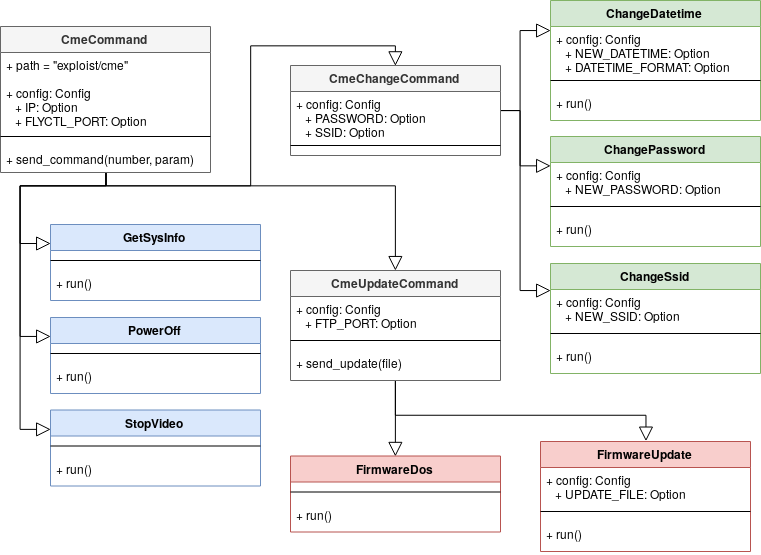
\includegraphics[width=\linewidth]{figures/dronesploit-modules}
  \caption{Dronesploit modules represented in a UML fashion}
  \label{fig:dronesploit-modules}
\end{figure}

All the modules rely on a base proxy class \texttt{CmeCommand} defining a \texttt{send\_command} method that allows to interact with drone's fly controller. The different sets of modules are represented with distinct colors :
\begin{itemize}
  \item \textbf{Information request modules} (in blue) : these directly subclass the \texttt{CmeCommand} and use a command index (as discovered in Subsection \ref{subsec:reverse-engineering}) with the \texttt{send\_command} method.
  \item \textbf{Setting change modules} (in green) : these subclass the \texttt{CmeChangeCommand} that adds some particular required config options for the drone command to work.
  \item \textbf{Firmware modules} (in red) :  these subclass the \texttt{CmeUpdateCommand} that defines a \texttt{send\_update} method to interact with FTP before triggering the actual update with the \texttt{send\_command} method.
\end{itemize}

The code hereafter demonstrates the logic of the aforementioned modules as of the information obtained in Chapter \ref{exploits}.

\paragraph{Modifying drone configuration} As described in Subsection \ref{subsec:sending-config-commands}, we were able to understand protocol used to modify a drone's configuration. It was then rather straightforward to develop a script that would send the same payload. We used a socket to establish a connection with the device. Then, we simply send the command. 

\begin{center}
\begin{lstlisting}[caption={Piece of code for sending a drone command}]
import socket

def send_command(ip, port, id, param):
    """
    :param ip:    drone's IP
    :param port:  drone's fly controller port
    :param id:    command identification number
    :param param: command set of parameters
    """
    s = socket.socket(socket.AF_INET, socket.SOCK_STREAM)
    s.connect((ip, port))
    s.send(b'{"CMD" : %d, "PARAM" : %s}' % (id, param))
    return s.recv(1024).strip() == b"0"
\end{lstlisting}\label{lst:dronesploit-drone-command}
\end{center}

As shown in Listing \ref{lst:dronesploit-drone-command}, simple TCP socket is required with drone's IP and port to send a dictionary holding the command identifying number and its parameters. Afterwards, drone's fly controller returns a value "\texttt{0}" for success and "\texttt{-1}" for failure.

\paragraph{Uploading modified firmware} Following the work of Subsection \ref{subsec:post-exploitation}, we were able to have a peek at the FTP commands necessary to open a connection and upload a new version of the firmware. Combined with the credentials discovered in the Subsection \ref{subsec:reverse-engineering}, we could successfully develop a script that allows to upload the modified version of the firmware to the drone, using a socket connection and a syntax analog to the module above.

\begin{center}
\begin{lstlisting}[caption={Piece of code for sending an evil firmware update}]
from ftplib import FTP

def send_update(ip, port, filename):
    ftp = FTP(ip, port)
    ftp.sendcmd("USER AW819")
    ftp.sendcmd("PASS 1663819")
    ftp.sendcmd("SYST")
    ftp.sendcmd("PWD")
    ftp.sendcmd("TYPE I")
    ftp.sendcmd("CWD /")
    ftp.sendcmd("PASV")
    with open(filename, 'rb') as f:
        ftp.storbinary("STOR 0.7.15.zip", f)
    ftp.quit()
    if send_command(ip, port, 71, '"0.7.15"'):
        time.sleep(10)
        return True
    return False
\end{lstlisting}\label{lst:dronesploit-firmware-update}
\end{center}

As shown in Listing \ref{lst:dronesploit-firmware-update}, we can simply open an FTP session and mimic the FTP commands as found in Subsection \ref{subsec:post-exploitation} to upload our evil firmware update. Then, we can send a drone command to trigger the actual update. If it succeeds, the update process takes roughly 10 seconds.

\paragraph{In-flight shutdown} As an additional note, when having enabled the Telnet service, it is trivial to send a shutdown command after establishing a connection to the drone through a terminal. This could be automated in a module in a near future.

\begin{tip}
As a reminder, the information request (in blue) and setting change (in green) modules apply to both the Flitt and the C-me. The set of firmware update commands only applies to the C-me.
\end{tip}

\begin{summary}
\textbf{Sploitkit}, written in Python, was recently created and provides a comprehensive framework for building terminal-based interfaces. It is designed with the \acrshort{dry} philosophy in mind and provides an \acrshort{api} that makes easy to create what are called \textit{entities}. These consist in :
\begin{itemize}
  \item \texttt{Console}'s : for building new console levels.
  \item \texttt{Command}'s : for creating commands for the consoles.
  \item \texttt{Module}'s : for making modules handling complex computation that do not fit into commands. 
  \item \texttt{Model}'s : for tuning the data schem of the internal store (useful for collecting report information).
\end{itemize}

Above this framework, we can now build an application called \textbf{DroneSploit} that is purely focused on our use case, drone hacking. For this purpose, we retrieve the knowledge acquired in Chapters \ref{scope} and \ref{exploits}. From this, we can essentially deduce two important logics :
\begin{enumerate}
  \item Send specifically formatted commands to the drones \newline (applies to the Flitt but to the C-me as well)
  \item Push a firmware update and trigger the update process \newline (only for the C-me)
\end{enumerate}

This led us to build the following \textbf{modules} :
\begingroup
\renewcommand*{\arraystretch}{1.3}
\begin{center}
\rowcolors{2}{gray!25}{white}
  \begin{tabular}{L{5cm}C{3cm}C{3.5cm}}
  \rowcolor{gray!50}
  \hf{5cm}{} & \hf{3cm}{Flitt Selfie Cam} & \hf{3.5cm}{C-me Selfie Drone} \\
  Get system information & \ding{51} & \ding{51} \\
  Power off & \ding{51} & \ding{51} \\
  Stop video recording & \ding{51} & \ding{51} \\
  Change datetime & \ding{51} & \ding{51} \\
  Change password & \ding{51} & \ding{51} \\
  Change SSID & \ding{51} & \ding{51} \\
  Evil firmware update & \ding{55} & \ding{51} \\
  Denial-of-Service update & \ding{55} & \ding{51} \\
  \end{tabular}
\end{center}
\endgroup

It was also possible to automate some \textbf{WiFi password cracking} techniques using available open source code, to be adapted in Sploitkit modules.

The resulting project can be found on GitHub. \cite{dronesploit}
\end{summary}

\begin{discussion}
While the exploitation phase had already become exciting, this one turned out to be inspiring. It dealed with more complex, parametrizable and repeatable logics in Python so that, at the end, we could write modules for a brand new application based on Sploitkit.

While creating modules, this paved the way to automating more and more possible ways of attack on a broad range of targets. Indeed, now that a basis is stated with DroneSploit, it will be relatively easy to add new modules for out-of-scope drones that are already parsed in the current literature, e.g. the Parrot AR or yet DJI Tello drones. This will be the subject of further exciting researches !

For the viewing pleasure, here is a screenshot of what DroneSploit currently looks like :

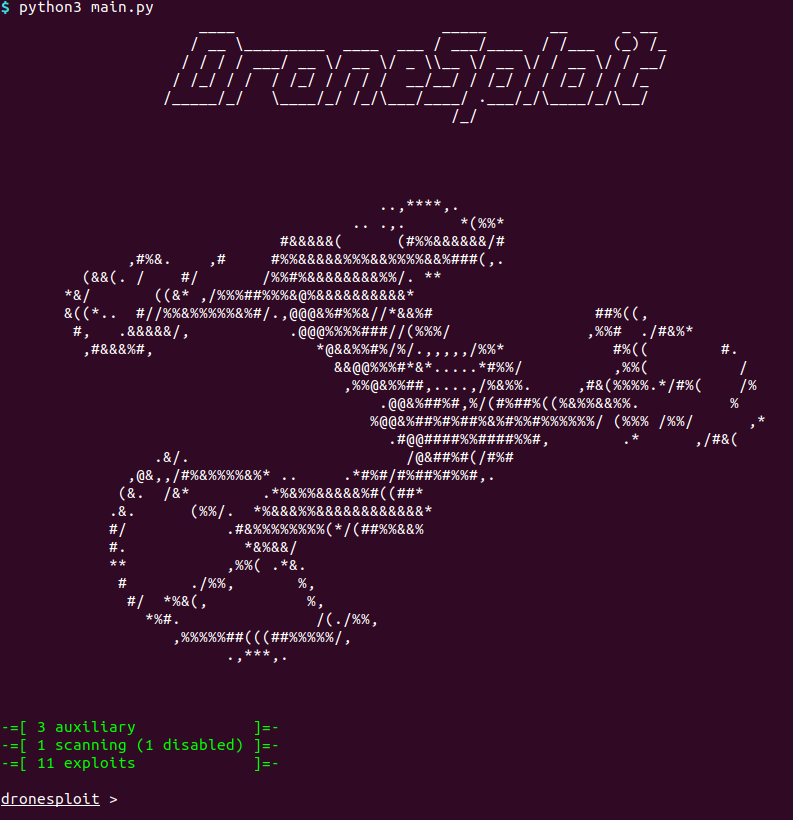
\includegraphics[width=\linewidth]{figures/dronesploit}

To be continued !
\end{discussion}

\end{chaptercover}

  \insertblankpage
  \begin{chaptercover}{Conclusion}%
{\coverepigraph{``Device makers, especially consumer-focused ones, have been the Achilles' heel of IoT security. These vendors have often viewed proper security implementations as extra cost, complexity, and time- to-market burdens with an unclear payoff."}{\textsc{Maciej Kranz} \newline {\normalsize\vspace{-.3cm}Vice President of Strategic Innovation at Cisco Systems}}
{\large \vspace{-1.5cm} \hyphenation{problem} \bigletter{A}{t first glance}, one could assume that a small commercial drone naturally lacks security. And by definition, a connected device will always be more vulnerable than one that is not. Although we were able to exploit the devices on unplanned ways to a certain extent, this still required a consequent amount of work.  \newline \\}}%
{conclusion}

\section{Summary}
All along this thesis, we dove into the very specific field of pentesting and vulnerability assessment. This process was a formidable journey that allowed us to have a good overview of every step involved in the discipline, by applying the offensive security techniques to the context of drones.

First, we got familiar with all the tools and technologies that could be of help for a pentester. This process was rather enjoyable and very instructive. The more we learned, the more we realized that the scope of cybersecurity is wide and complex.

Afterwards, we dove into the specifics of drone security, limited the scope to two models of drones, and established a quick state of the art of the topic. Followed an intelligence gathering and vulnerability scanning phase that allowed us to pinpoint some vulnerabilities for each one of the devices. Strong with this knowledge we developed a process that allowed us to gain full access to the drone, and even to install a backdoor.

Finally, we designed and implemented a framework from scratch, DroneSploit. It is designed to automate the exploits for which we managed to determine a proof of concept in the previous phase. The framework is designed in such a way that it mimics Metasploit, the reference toolkit for network penetration testing, with hopes that other security enthusiasts would be interested to contribute to the project.

The result of this work, after considering the fact that success was no a certainty from the beginning, has proven to be rewarding.  

\section{Objectives}
Our objectives were four-fold :
{\hyphenation{}
\begin{enumerate}[itemsep=0.1cm,topsep=0.1cm]
  \item The \textbf{background} is fully stated.
  \begin{enumerate}[label=\Alph* --,align=left,itemsep=.05cm,topsep=0.1cm]
    \item We reviewed the current literature regarding IoT security, especially in the field of light commercial drones.
    \item We found some methodologies and processes for hacking, especially the penetration testing process.
    \item We presented some existing solutions and used a few ones in the exploits and the framework.
  \end{enumerate}
  \item The \textbf{scope} was narrowed to only two drones.
  \begin{enumerate}[label=\Alph* --,align=left,itemsep=.05cm,topsep=0.1cm]
    \item Multiple provided drones were not suitable for WiFi exploitation and then withdrawn from the scope.
    \item The working of the selected drones was studied.
  \end{enumerate}
  \item Some \textbf{exploits} could be written and tested.
  \begin{enumerate}[label=\Alph* --,align=left,itemsep=.05cm,topsep=0.1cm]
    \item We found a few attacks chaining multiple hacking techniques.
    \item We wrote a few exploit scripts proven to be effective.
  \end{enumerate}
  \item A new \textbf{framework} is born, tailored to drone hacking.
  \begin{enumerate}[label=\Alph* --,align=left,itemsep=.05cm,topsep=0.1cm]
    \item The new framework was made on top of SploitKit and some scanning modules could be included.
    \item The exploit scripts were turned into exploitation modules for DroneSploit.
  \end{enumerate}
\end{enumerate}}

\section{Future Works} \label{sec:future-works}
DroneSploit opens some new avenues of improvement :
{\hyphenation{}
\begin{itemize}[itemsep=0.02cm,topsep=0.02cm]
  \item \textbf{Flying control module} : using the information gathered in the Subsection \ref{subsec:traffic-analysis}, it should be possible to design a light control application in order to pilot the drone from a distance. 
  \item \textbf{Video eavesdropping} : it might be worthwhile to try to intercept the video communication between the drone and the smartphone. If so, this functionality could be conveniently used as a nice addition to the flying control module.
  \item \textbf{Radio-controlled drone assessment} : even though we excluded them from the scope of this work, there are a lot of commercial drones that are radio controlled. It would be worthwhile to study them as a separate project, and see there is a possible application with DroneSploit.
  \item \textbf{Testing other drone models} : increase the number of modules available in DroneSploit by realizing a similar work with some more light commercial drones, or by adding scripts already available as resources
  \item \textbf{Evolving to medium-size drones} :  this work focus on rather inexpensive devices. It would be worthwhile to test some bigger models, and see if more security is implemented.
\end{itemize}}

\end{chaptercover}

  \setcounter{chapter}{0}
  \addtocontents{toc}{\protect\setcounter{tocdepth}{0}} % for other parts (i.e. appendices), do not count sections, subsections, ...
  \addtocontents{ptc}{\protect\setcounter{tocdepth}{2}} % but for appendices' toc's, keep depth to 2
  %\addtocontents{toc}{\protect\newpage}
  \insertblankpage
  %\bibliographystyle{IEEEtran}
%\cite{*}
%\bibliography{parts/bibliography}
%\newpage

\nocite{*}
\printbibliography[heading=bibintoc,title={\textbf{References}}]
\newpage

  \def\xshiftfactor{.53} % scaling factor for positioning chapter number label (set to .525 for numbered chapters)
  \appendix
  \insertblankpage
  \specialinclude{appendices/wifi-cracking}{Cracking WPA2-PSK WiFi using Aircrack-ng}{app:wifi-cracking}
  \insertblankpage
  \specialinclude{appendices/uart-pins}{UART pins}{app:uart-pins}
\end{document}